%% BioMed_Central_Tex_Template_v1.06
%%                                      %
%  bmc_article.tex            ver: 1.06 %
%                                       %

%%IMPORTANT: do not delete the first line of this template
%%It must be present to enable the BMC Submission system to
%%recognise this template!!

%%%%%%%%%%%%%%%%%%%%%%%%%%%%%%%%%%%%%%%%%
%%                                     %%
%%  LaTeX template for BioMed Central  %%
%%     journal article submissions     %%
%%                                     %%
%%          <8 June 2012>              %%
%%                                     %%
%%                                     %%
%%%%%%%%%%%%%%%%%%%%%%%%%%%%%%%%%%%%%%%%%

%%%%%%%%%%%%%%%%%%%%%%%%%%%%%%%%%%%%%%%%%%%%%%%%%%%%%%%%%%%%%%%%%%%%%
%%                                                                 %%
%% For instructions on how to fill out this Tex template           %%
%% document please refer to Readme.html and the instructions for   %%
%% authors page on the biomed central website                      %%
%% https://www.biomedcentral.com/getpublished                      %%
%%                                                                 %%
%% Please do not use \input{...} to include other tex files.       %%
%% Submit your LaTeX manuscript as one .tex document.              %%
%%                                                                 %%
%% All additional figures and files should be attached             %%
%% separately and not embedded in the \TeX\ document itself.       %%
%%                                                                 %%
%% BioMed Central currently use the MikTex distribution of         %%
%% TeX for Windows) of TeX and LaTeX.  This is available from      %%
%% https://miktex.org/                                             %%
%%                                                                 %%
%%%%%%%%%%%%%%%%%%%%%%%%%%%%%%%%%%%%%%%%%%%%%%%%%%%%%%%%%%%%%%%%%%%%%

%%% additional documentclass options:
%  [doublespacing]
%  [linenumbers]   - put the line numbers on margins

%%% loading packages, author definitions

%\documentclass[twocolumn]{bmcart}% uncomment this for twocolumn layout and comment line below
\documentclass{bmcart}

%%% Load packages
%\usepackage{amsthm,amsmath}
%%\RequirePackage[numbers]{natbib}
%%\RequirePackage[authoryear]{natbib}% uncomment this for author-year bibliography
%%\RequirePackage{hyperref}
%\usepackage[utf8]{inputenc} %unicode support
%%\usepackage[applemac]{inputenc} %applemac support if unicode package fails
%%\usepackage[latin1]{inputenc} %UNIX support if unicode package fails

\usepackage{amsthm,amsmath}
\usepackage{amsfonts}
\usepackage{graphicx}
\usepackage[utf8]{inputenc}

\usepackage{todonotes}
\usepackage{lmodern}  % font sizes
\usepackage{hyperref} % ref unlabeled sections
\usepackage{subcaption}

%%%%%%%%%%%%%%%%%%%%%%%%%%%%%%%%%%%%%%%%%%%%%%%%%
%%                                             %%
%%  If you wish to display your graphics for   %%
%%  your own use using includegraphic or       %%
%%  includegraphics, then comment out the      %%
%%  following two lines of code.               %%
%%  NB: These line *must* be included when     %%
%%  submitting to BMC.                         %%
%%  All figure files must be submitted as      %%
%%  separate graphics through the BMC          %%
%%  submission process, not included in the    %%
%%  submitted article.                         %%
%%                                             %%
%%%%%%%%%%%%%%%%%%%%%%%%%%%%%%%%%%%%%%%%%%%%%%%%%

%\def\includegraphic{}
%\def\includegraphics{}

%%% Put your definitions there:
\startlocaldefs
\newcommand{\lyxdot}{.}
\endlocaldefs

%%% Begin ...
\begin{document}

%%% Start of article front matter
\begin{frontmatter}

\begin{fmbox}
\dochead{Research}

%%%%%%%%%%%%%%%%%%%%%%%%%%%%%%%%%%%%%%%%%%%%%%
%%                                          %%
%% Enter the title of your article here     %%
%%                                          %%
%%%%%%%%%%%%%%%%%%%%%%%%%%%%%%%%%%%%%%%%%%%%%%

%\title{Prediction of Protein-Protein Interactions on the Human and Rice Interactomes}
\title{Protein-Protein Interaction Prediction based on Interactome Connectivity}

%%%%%%%%%%%%%%%%%%%%%%%%%%%%%%%%%%%%%%%%%%%%%%
%%                                          %%
%% Enter the authors here                   %%
%%                                          %%
%% Specify information, if available,       %%
%% in the form:                             %%
%%   <key>={<id1>,<id2>}                    %%
%%   <key>=                                 %%
%% Comment or delete the keys which are     %%
%% not used. Repeat \author command as much %%
%% as required.                             %%
%%                                          %%
%%%%%%%%%%%%%%%%%%%%%%%%%%%%%%%%%%%%%%%%%%%%%%

\author[
  addressref={aff1},                   % id's of addresses, e.g. {aff1,aff2}
  corref={aff1},                       % id of corresponding address, if any
% noteref={n1},                        % id's of article notes, if any
  email={nicolaslopez@javerianacali.edu.co}   % email address
]{\inits{N.L.}\fnm{Nicolás A.} \snm{López-Rozo}}
\author[
  addressref={aff1},
  email={jfinke@javerianacali.edu.co}
]{\inits{J.F.}\fnm{Jorge} \snm{Finke}}
\author[
  addressref={aff1},
  email={camilo.rocha@javerianacali.edu.co}
]{\inits{C.R.}\fnm{Camilo} \snm{Rocha}}

%%%%%%%%%%%%%%%%%%%%%%%%%%%%%%%%%%%%%%%%%%%%%%
%%                                          %%
%% Enter the authors' addresses here        %%
%%                                          %%
%% Repeat \address commands as much as      %%
%% required.                                %%
%%                                          %%
%%%%%%%%%%%%%%%%%%%%%%%%%%%%%%%%%%%%%%%%%%%%%%

\address[id=aff1]{%                           % unique id
  \orgdiv{Department of Electronics and Computer Science},             % department, if any
  \orgname{Pontificia Universidad Javeriana},          % university, etc
  \city{Cali},                              % city
  \cny{CO}                                    % country
}


%%%%%%%%%%%%%%%%%%%%%%%%%%%%%%%%%%%%%%%%%%%%%%
%%                                          %%
%% Enter short notes here                   %%
%%                                          %%
%% Short notes will be after addresses      %%
%% on first page.                           %%
%%                                          %%
%%%%%%%%%%%%%%%%%%%%%%%%%%%%%%%%%%%%%%%%%%%%%%

%\begin{artnotes}
%%\note{Sample of title note}     % note to the article
%\note[id=n1]{Equal contributor} % note, connected to author
%\end{artnotes}

\end{fmbox}% comment this for two column layout

%%%%%%%%%%%%%%%%%%%%%%%%%%%%%%%%%%%%%%%%%%%%%%%
%%                                           %%
%% The Abstract begins here                  %%
%%                                           %%
%% Please refer to the Instructions for      %%
%% authors on https://www.biomedcentral.com/ %%
%% and include the section headings          %%
%% accordingly for your article type.        %%
%%                                           %%
%%%%%%%%%%%%%%%%%%%%%%%%%%%%%%%%%%%%%%%%%%%%%%%

\begin{abstractbox}

\begin{abstract} % abstract

\parttitle{Background} %if any
Abstract A recent study in network-based prediction of protein-protein interactions (PPIs) reveals that two proteins are more likely to interact, the higher the number of paths of length 3 between them (normalized by the geometric average of their interactions). This paper extends previous work on mapping binary interactions by taking into account the learning of features (embeddings) of the PPI network. In particular, we implement a gradient boosted decision tree model (XGBoost) using handcrafted features (including the normalized measure) and embeddings from an algorithm that generates a low-dimensional representation of nodes (node2vec).

\parttitle{Results} %if any
Our main result shows that while the measure remains an important feature for predicting interactions, better performance is achieved when in addition embedding features are considered. The proposed approach is validated for the human and rice interactomes. For both cases, the combination of both types of features yield higher AUC values.

\parttitle{Conclusions} %if any
As found on this study on both human and rice, when information from handcrafted features based on neighborhood is enhanced with vector representations from random walks, the prediction power of the model improves. Besides, a supervised learning model can be trained for predicting unknown interactions based on such information. Finally, the developed framework can also be applied to interactomes of other organisms for which PPI networks have recently become available.

\end{abstract}

%%%%%%%%%%%%%%%%%%%%%%%%%%%%%%%%%%%%%%%%%%%%%%
%%                                          %%
%% The keywords begin here                  %%
%%                                          %%
%% Put each keyword in separate \kwd{}.     %%
%%                                          %%
%%%%%%%%%%%%%%%%%%%%%%%%%%%%%%%%%%%%%%%%%%%%%%

\begin{keyword}
\kwd{PPI}
\kwd{Prediction of Protein Interaction}
\kwd{Machine Learning}
\kwd{Python}
\kwd{XGBoost}
\kwd{node2vec}
\end{keyword}

% MSC classifications codes, if any
%\begin{keyword}[class=AMS]
%\kwd[Primary ]{}
%\kwd{}
%\kwd[; secondary ]{}
%\end{keyword}

\end{abstractbox}
%
%\end{fmbox}% uncomment this for two column layout

\end{frontmatter}

%%%%%%%%%%%%%%%%%%%%%%%%%%%%%%%%%%%%%%%%%%%%%%%%
%%                                            %%
%% The Main Body begins here                  %%
%%                                            %%
%% Please refer to the instructions for       %%
%% authors on:                                %%
%% https://www.biomedcentral.com/getpublished %%
%% and include the section headings           %%
%% accordingly for your article type.         %%
%%                                            %%
%% See the Results and Discussion section     %%
%% for details on how to create sub-sections  %%
%%                                            %%
%% use \cite{...} to cite references          %%
%%  \cite{koon} and                           %%
%%  \cite{oreg,khar,zvai,xjon,schn,pond}      %%
%%                                            %%
%%%%%%%%%%%%%%%%%%%%%%%%%%%%%%%%%%%%%%%%%%%%%%%%

%%%%%%%%%%%%%%%%%%%%%%%%% start of article main body
% <put your article body there>

%%%%%%%%%%%%%%%%
%% Background %%
%%
\section*{Introduction}

Proteins are key actors of biological processes inside cells. Rather
than carrying out tasks as single agents, they are part of dynamic
networks of protein-protein interactions (PPI) \cite{Lin2017}. Such
networks underlie a variety of interdependent mechanisms, including
signal transduction, homeostasis control and stress responses. Furthermore,
PPI networks play an important role in physiological and developmental
processes such as protein phosphorylation, transcriptional co-factor
recruitment and transporter activation \cite{Zhang2010PPI}.

A common way to create PPI networks (or validate particular protein-protein
interactions) is the \emph{Yeast-Two-Hybrid} technique (also known
as \emph{two-hybrid screening} or \emph{Y2H}). Figure \ref{Y2H}A
illustrates the biological basis of Y2H: the expression of a specific
reporter gene is activated by the binding of a DNA-binding Domain
(DB) and an Activation Domain (AD) of a Transcription Factor, which
in turn binds to an Upstream Activation Sequence (UAS). To evaluate
an interaction between two proteins, the Y2H approach fuses one protein
to the DB domain (known as \emph{bait}) and another protein to the
AD (known as \emph{prey}). If the proteins interact, the reporter
gene expression is activated by the AD (Fig. \ref{Y2H}B). Otherwise,
if proteins fail to interact, the reporter gene is not expressed (Fig.
\ref{Y2H}C).

\begin{figure}[h]
\caption{\label{Y2H}The Yeast-2-Hybrid technique offers an experimental approach
for constructing PPI networks.}

%\noindent \centering{}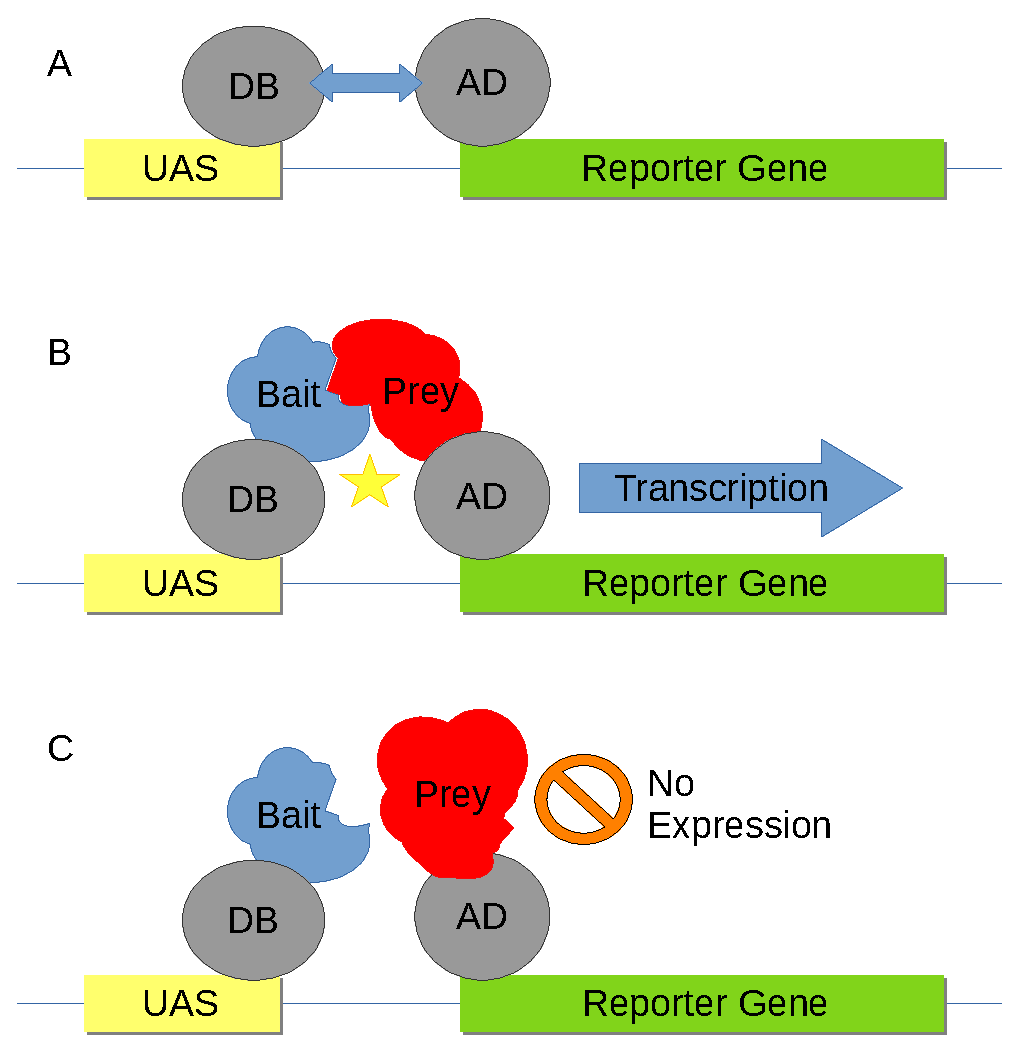
\includegraphics[width=0.7\columnwidth]{Y2H}
\end{figure}

Based on the outcome of numerous Y2H experiments, undirected networks
of interactions between proteins can be constructed. However, relying
only on experimental validation of PPIs is detrimental to research
due to its hindrance in costs, accuracy, required manpower and time
\cite{Laraia2015PPI,Macalino2018PPI}. Besides, the number of missing
interactions for pairs of proteins on many organisms leverage the
usage of computational methods for prediction of such interactions.

A common way of predicting interactions is usually based on social
networks analysis, more specifically on the triadic closure principle
(TCP). TCP states that the higher the number of common neighboring
nodes between two nodes, the higher the probability that they interact
\cite{Goldberg2003SmallWorld}. TCP can be addressed mathematically
by counting the number of shared neighbors of a pair of nodes, also
known as the Common Neighbors algorithm. By raising the adjacency
matrix (A) of the network to the second power (A\texttwosuperior ),
TCP can be considered for further analyses. However, previous studies
show that the mentioned approach usually fails because it does not
consider the structural and chemical properties of the proteins \cite{Cannistraci2013Networks,Kovacs2019}.

A variety of methods for predicting interactions in PPI networks have
been proposed in recent years \cite{Chang2016PPI,Chen2019PPI,Kotlyar2015PPI}.
Kovacs et al (2019) introduce a network-based approach which predicts
the interaction between two proteins based on the number of paths
of length 3, normalized by the geometric average of their interactions.
The simplest mathematical representation of this principle consists
on the third power of the adjacency matrix (A\textthreesuperior).
Furthermore, Kovacs et al present a degree-normalized scaling for
this metric, which reduces bias caused by intermediate hubs within
the paths of length 3. This handcrafted measure, denoted L3, enables
the proposed approach to outperform previous methods for predicting
binary protein interactions in yeast (\emph{S. cerevisiae}), Arabidopsis
(\emph{A. thaliana}), worm (\emph{C. elegans}), fly (\emph{D. melanogaster}),
fission yeast (\emph{S. pombe}), mouse (\emph{M. musculus}) and humans
\cite{Kovacs2019}.


The focus of this study is to evaluate different methods for predicting
PPIs using the network of known interactions. To achieve this, human
and rice PPI networks are compared using the proposed methods (A2,
A3, L3), as well as a low-dimensional representation of nodes (\texttt{Node2Vec})\cite{Grover_2016}.
After that, combinations of the two types of methods are tested. In
the case of the human network, two different versions of the human
interactome \cite{Rolland2014Human} are used for training and another
interactome version is used for validation (\emph{HI-III})\cite{Kovacs2019}.
For the rice interactome, a portion of the known interactions removed
and then predicted with different techniques based on the known interactions.
The main contributions of this paper are i) a general framework for
link prediction in non-directed networks and ii) two applications
of this framework to biological networks with a structural insight.

\paragraph*{Structure:} This paper is organized as follows. \emph{Materials and Methods} describes
the methodological steps and key milestones in the preparation of
the networks, model parameters and experimental configurations.
\emph{Results} presents the main results of the models for the human and rice interactomes.
\emph{Conclussions} presents the main conclusions of this study. Finally, \emph{Appendix}
presents supplementary information and figures which complement the
results described in this paper.

\section*{Preliminaries}

% "Preliminaries" refers to fundaments for the new reader on the main topics of
% the paper

Let $G=(V,E), n=|V|, m=|E|$ be an undirected graph describing $n$
proteins and $m$ pairwise interactions between them. $G$ can be represented as a Boolean 
adjacency matrix $A$ of size $n\cdot n$, where the value for a position
$(i,j), 0\leq i,j < n$ is set to $1$ if there is a direct interaction
between proteins $i$ and $j$, or set to $0$ otherwise. As it is an undirected network, $A$ is symmetric.

Given this matrix $A$, to find the number of paths of exactly $k$ steps  in the network, $A$ can be raised to the \textit{k}-th power. 

\section*{Prediction Framework}

% Model framework - similar to materials and methods, but with more paragraph
% continuity

\subsection*{Framework Conception and Configuration}

As mentioned before, the functionality of a protein strongly depends on its 3D structure, 
so that changes in its conformation (mutations) can affect how a protein interacts with its 
surroundings \cite{Sikosek2014Prot}. In this aspect, $A_G$ gives intrinsic information 
about complementarity between pairs of proteins and hence paths on the protein network are 
relevant for the prediction task. 

The proposed framework for prediction of protein-protein interactions consists of the
combination of the path counting metrics along with the vector representations of the
edges of the network (node2vec embeddings). Namely, the path counting metrics are either 
the counting of paths of length 2 (matrix $A_G^2$), the counting of paths of length 3 
(matrix $A_G^3$) or the degree-normalized counting of paths of length 3 (matrix $L_3$). 
The information retrieved from these matrices will be addressed from now on as A2, A3 
and L3, respectively.

Figure \ref{fig:framework} shows the proposed framework for predicting protein-protein interactions. As the 
framework combines two sources of information, it consists of three processes: (a) Metrics 
calculation and initial predictions, (b) Node and edge embeddings and (c) Machine Learning 
prediction.

\begin{figure}[h]
\caption{\label{fig:framework}Framework scheme}
	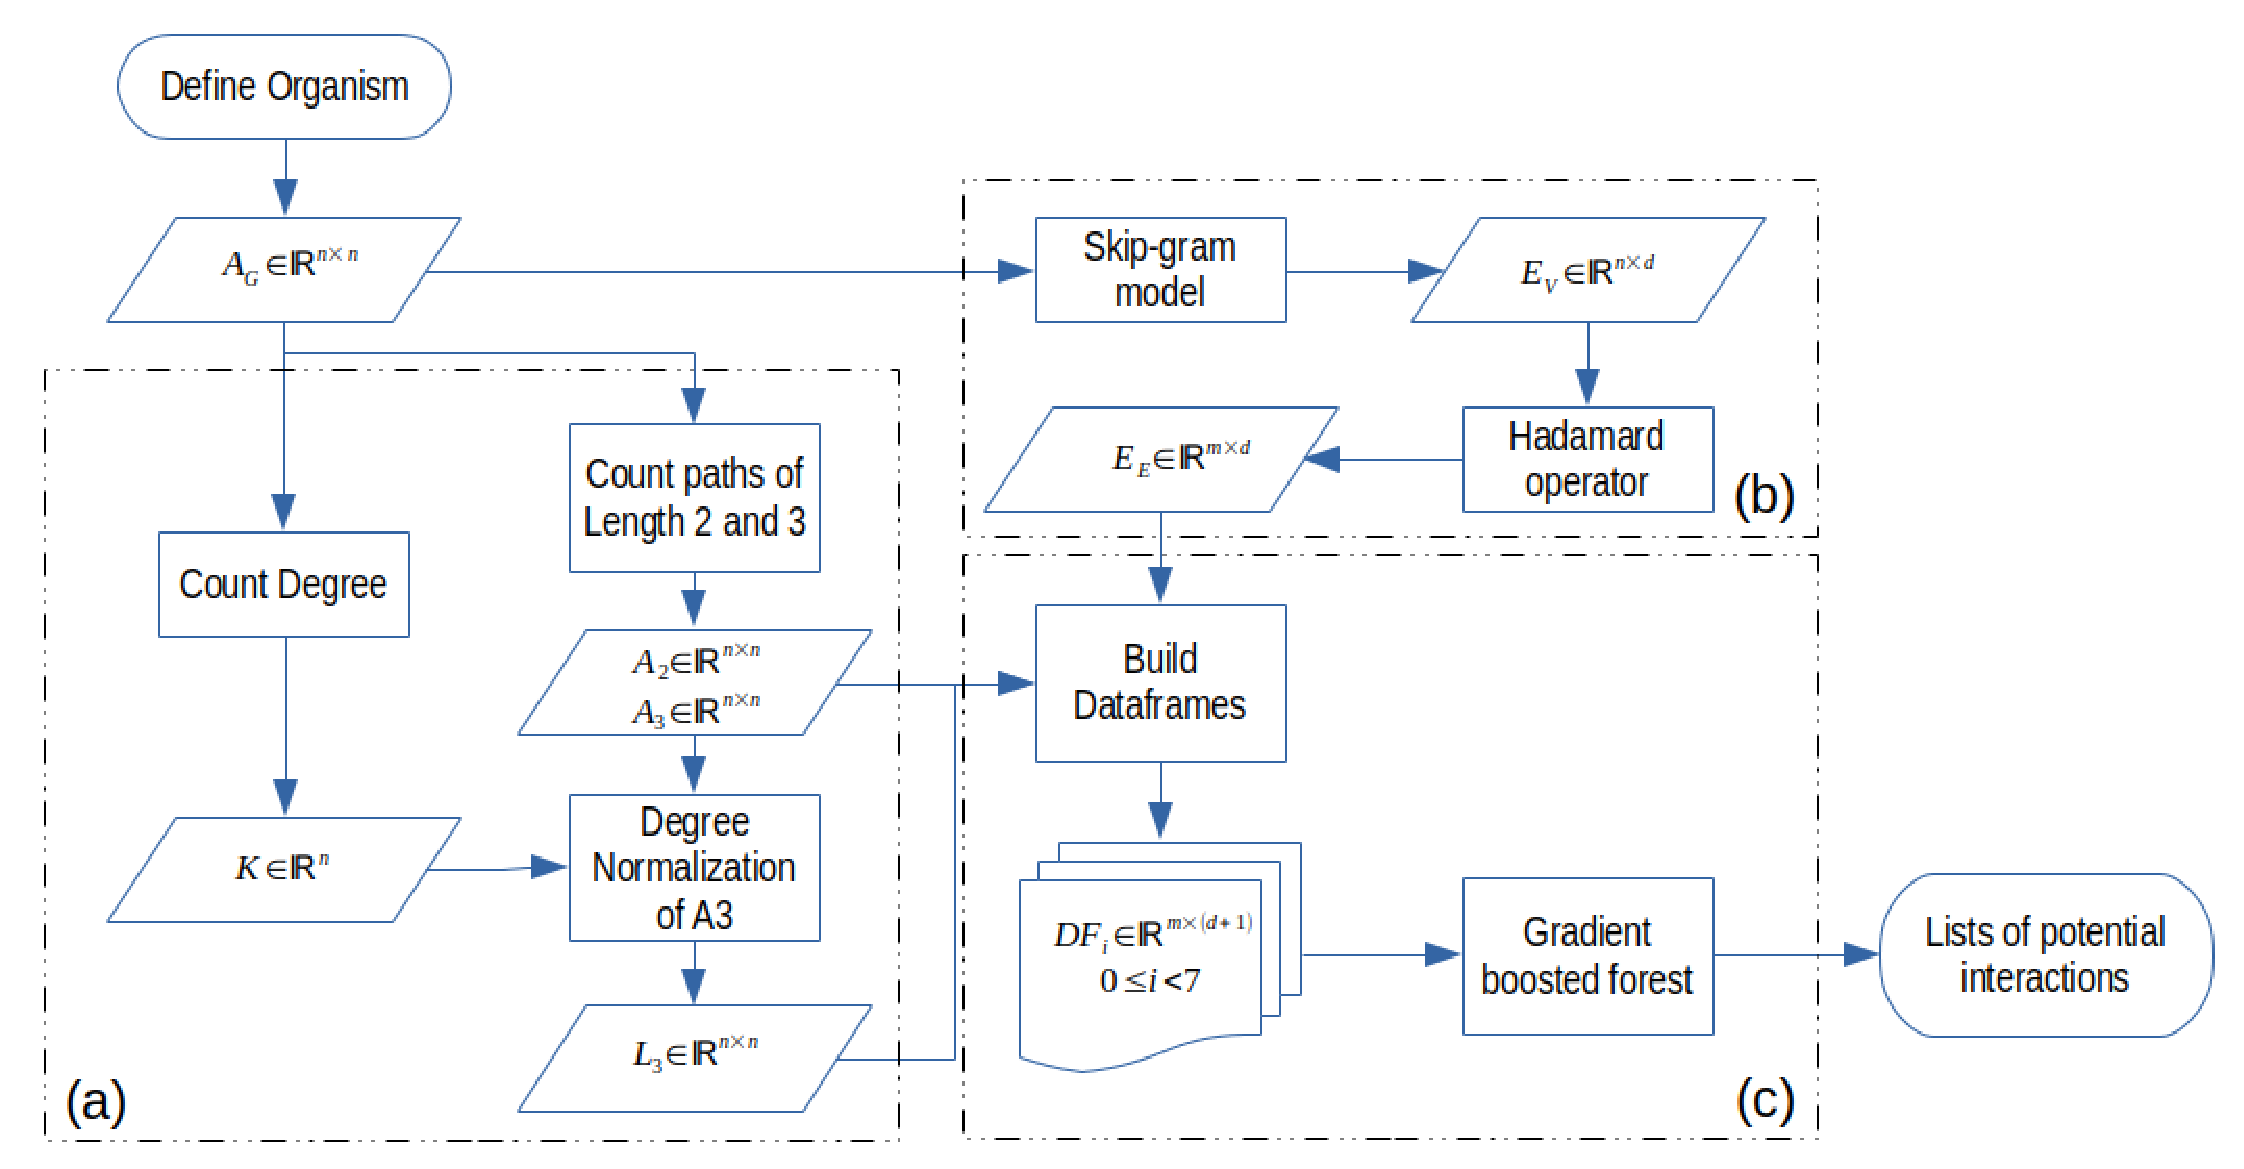
\includegraphics[width=\textwidth ]{figures/framework.eps}
\end{figure}

The input for the workflow consists of a representation of the connectivity of the network.
Online databases of protein-protein interactions usually report this information as an 
adjacency list with some additional attributes about the quality of this interaction. Namely, 
this data is represented as a list of pairs of identifiers and zero or more attributes for 
each pair. The framework only needs to know whether an interaction exists and therefore this 
additional information needs to be discarded in advance. In order to calculate optimally the
subsequent metrics, the framework creates the adjacency matrix $A_G$ out of the given list. 
Note that as no attributes from nodes or edges are added, the framework predicts based only 
on the intrinsic properties of the network related to connectivity. 

\subsubsection*{A. Metrics Calculation}
The goal of this stage is to build matrices $A2$, $A3$ and $L3$ which quantify, 
the number of paths of length 2, of length 3 and the degree-normalized count of 
paths of length 3, respectively. For this purpose, two calculations are done: 
counting the degree of each node ($k_i \in \mathbb{Z}$) and raising $A_G$ to the 
second to obtain $A2$. Finally, $A3$ and $L3$  are calculated simultaneously. 
Entries $L3_{i,j}$ of $L3$ can be calculated as 

\begin{equation}
  L3_{i,j}=\sum_{p,q\in V}\frac{{A_G}_{i,p}\cdot {A_G}_{p,q}\cdot {A_G}_{q,j}}{\sqrt{k_{p}\cdot k_{q}}}
\end{equation}

\subsubsection*{B. node2vec Embeddings}
The purpose of this step is to retrieve a vector representation of the network 
structure and thus be able to feed the Machine Learning model and improve its 
predictions. This is done using a state-of-the-art algorithm called node2vec, 
which is based on the word2vec technique to learn learn word associations from
a corpus of text. Instead of sentences, node2vec uses 
random walks from each node in order to construct a skip-gram model and a neural 
network to learn features (embeddings) from the nodes\cite{Grover_2016}. These 
features consist of a $d$-dimensional vector representation of each node.
Since the framework aims to predict edges, these node embeddings are used as 
input for the Hadamard operator to calculate edge embeddings. Namely, the edge 
embedding of edge $c_i,j$ is calculated as the element-wise product of each 
component of the node embeddings for nodes $i$ and $j$. $d$ is chosen as 16.

\subsubsection*{C. Machine Learning Prediction}
Finally, this stage aims at gathering information from the previous steps to 
enrich the prediction of a Machine Learning (ML) model and improve its results. 

The selected implementation for this prediction problem is XGBoost, which 
uses gradient boosted decision trees to learn whether an interaction is feasible. 
The first step in this process is to combine the two sources of information into 
Dataframes for each of the metrics: for each edge, the information from one of the 
metrics (A2, A3 or L3) is appended to the vector representation of $d$ dimensions 
from node2vec, resulting in 3 different tables. Dataframes including only one 
source of information (each metric or node2vec data) are also generated and 
fed to XGBoost for comparison.

For each metric, the initial prediction in step A is used to train the supervised 
ML model 


\subsection*{Framework Evaluation on the Human Interactome}

As the first step in the evaluation of A2, A3 and L3 metrics to assess link
prediction, the full calculation and ranking of all predictions was
carried out. The results for the analyzed human interactomes (\emph{HI-II-14}
and \emph{HI-TESTED}) is shown in Figure \ref{fig:HI1}, in which
the x axis represents a rank position $k$ and the y axis displays
the precision for the top $k$ predictions of each method, when assuming
interactome \emph{HI-III} as the validation set. 
	
\begin{figure}[h]
\caption{\label{fig:HI1}Methods Comparison for \emph{HI-II-14} and \emph{HI-TESTED}}
	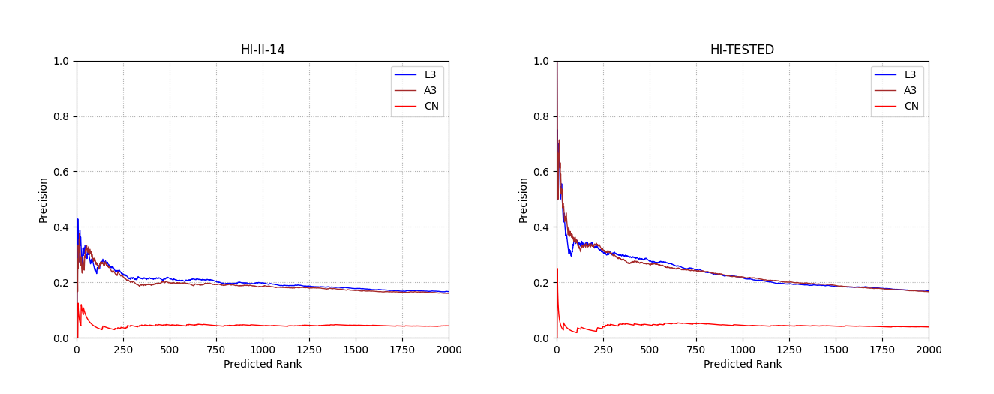
\includegraphics[width=\textwidth ]{figures/figure2.eps}
	%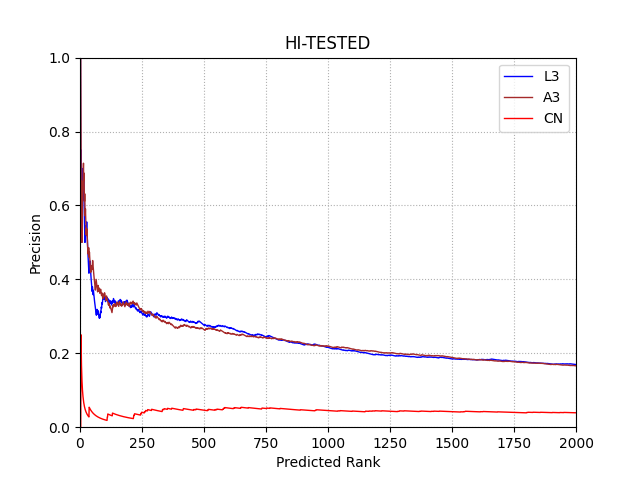
\includegraphics[width=0.7\textwidth ]{../hi-tested.txt.}
\end{figure}

As it can be inferred from the plots, L3-based predictions outperform
their $A{{}^2}$ counterparts. Results also show that L3-score and
$A^{3}$predictions follow a very similar trend.

However, the interest of this study is to assess if Machine Learning can boost
the overall performance on the prediction, so the proposed procedure
is adapted to the human interactome data: Instead of having to remove
a fraction of edges from the network in order to predict and validate,
the prediction network and the validation networks are given beforehand.
The rest of the procedure is carried out as mentioned above.
Table \ref{T1} presents the results for the combinations of Node2Vec
with each feature.

\begin{table}
\caption{\label{T1}Summary statistics for human interactomes}
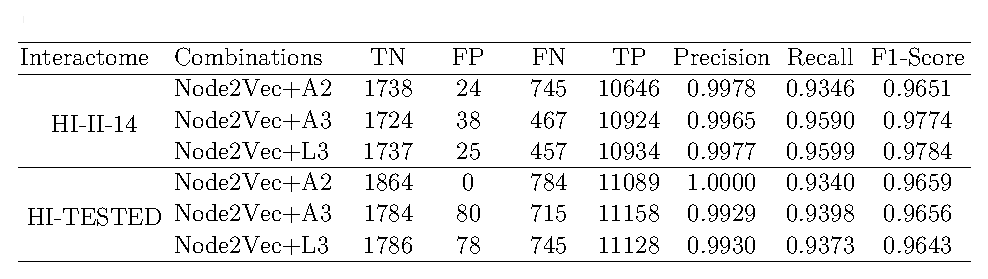
\includegraphics[width=1\columnwidth]{figures/T1}
\end{table}

In general, performance of all models is above 0.96 in terms of F1-Score.
Although marginally, the A2 feature-enriched model for HI-TESTED performs
better than their counterparts based on paths of length 3. The opposite
is also true for HI-II-14: models enriched with L3 and A3 features
perform better than their A2 counterpart. Results for the Interactome
\emph{HI-II-14} with Node2Vec and each metric are presented in Figures
S\ref{HI1}, S\ref{HI2} and S\ref{HI3}. It can be seen that for
\emph{HI-II-14}, A2 performs marginally better than L3 when comparing
precision but worse in terms of recall, although all metrics have
AUC values of 0.99.

On the other hand, the interactome \emph{HI-TESTED} was assessed with
the same methodology as \emph{HI-II-14} and results are shown in Figures
S\ref{HI1-1}, S\ref{HI2-1} and S\ref{HI3-1}. For this interactome,
A2 performs better in terms of false positives than A3 and L3, but
in terms of false negatives, A3 actually performs better that A2 and
L3. In terms of AUC, metrics results are indistinguishable. 

An interesting assessment from this human datasets can be observed
when looking at the importance plots, which show a very biased influence
of the handcrafted features. Figure \ref{F8-importance-H1} shows
this behavior for the \emph{HI-II-14} dataset, which is very similar
to \emph{HI-TESTED} (Figure S\ref{F8-importance-H2}).

\begin{figure}[h]
\noindent \begin{centering}
\caption{\label{F8-importance-H1}Importance gain plots for \emph{HI-II-14}}
\par\end{centering}
\begin{centering}
\includegraphics[width=0.48\columnwidth]{figures/Human/Imp\lyxdot A2\lyxdot 1\lyxdot eps}\includegraphics[width=0.48\columnwidth]{figures/Human/Imp\lyxdot A3\lyxdot 1\lyxdot eps}
\par\end{centering}
\centering{}\includegraphics[width=0.48\columnwidth]{figures/Human/Imp\lyxdot L3\lyxdot 1}
\end{figure}

\section*{Case Study: Rice Interactome Exploration}

%\section*{Results}
\section*{Identifying Potential Saline Stress Responsive Genes in Rice}
\label{sec.case}

This section presents a case study, applying the approach introduced in 
\hyperref[sec.framework]{the Workflow} section, to identify genes in
\textit{Oryza sativa} that respond to saline stress.
\vspace{0.5cm}

The RNA-seq data are available from the
GEO database \cite{clough2016gene} (accession
number GSE98455). It corresponds to $n_0=57\,845$ gene
expression profiles of shoot tissues measured for control and
salt conditions in $m=92$ accessions of the Rice Diversity Panel 1~\cite{eizenga2014registration},
with $r=2$ biological replicates. A total of $p=3 $ phenotypic traits
are used: shoot $K$ content, root biomass, and shoot biomass. These
traits were measured for the same $92$ genotypes, under control and
treatment conditions, and can be found in the supplementary
information for~\cite{campbell2017allelic}.

\subsection*{A. Data Pre-processing}

DESeq2 normalization is applied to the raw data and the biological
replicates are averaged. Genes exhibiting low variance are
identified as those with ratio of upper quantile to lower quantile
smaller than $1.5$ and are removed from the normalized data. Genes
with low expression, corresponding to those having more than $80\%$
samples with values smaller than $10$, are also removed. After this
filtering process a total of $n_1 = 9\,414$ genes are kept for further analysis.
\vspace{0.5cm}

From the Log Fold Change matrix $L_0$, genes whose difference between
upper quantile and lower quantile is greater than $0.25$ are
removed. Therefore, the resulting matrix $L_1$ contains the log ratios
of $n_2 = 8\,928$ genes. The logarithmic ratios of the phenotypic data,
for the $92$ accessions and the $3$ traits, are also computed.

\subsection*{B. Construction of the Co-expression Network}

The Log Fold Change matrix $L_1$ is used to compute the corresponding
similarity matrix.  For this network, it is observed that $\beta=3$ is
the smallest integer such that the $R^2 \geq 0.8
$. Figure~\ref{fig:beta} depicts the degree distribution of the
similarity matrix (left) and the degree distribution of the adjacency
matrix (right), which is the degree distribution of a scale-free
network with $R^2 = 0.8$ with $\beta = 3$.
\vspace{0.5cm}

%figure 2
\begin{figure}[htbp]
  \centering
    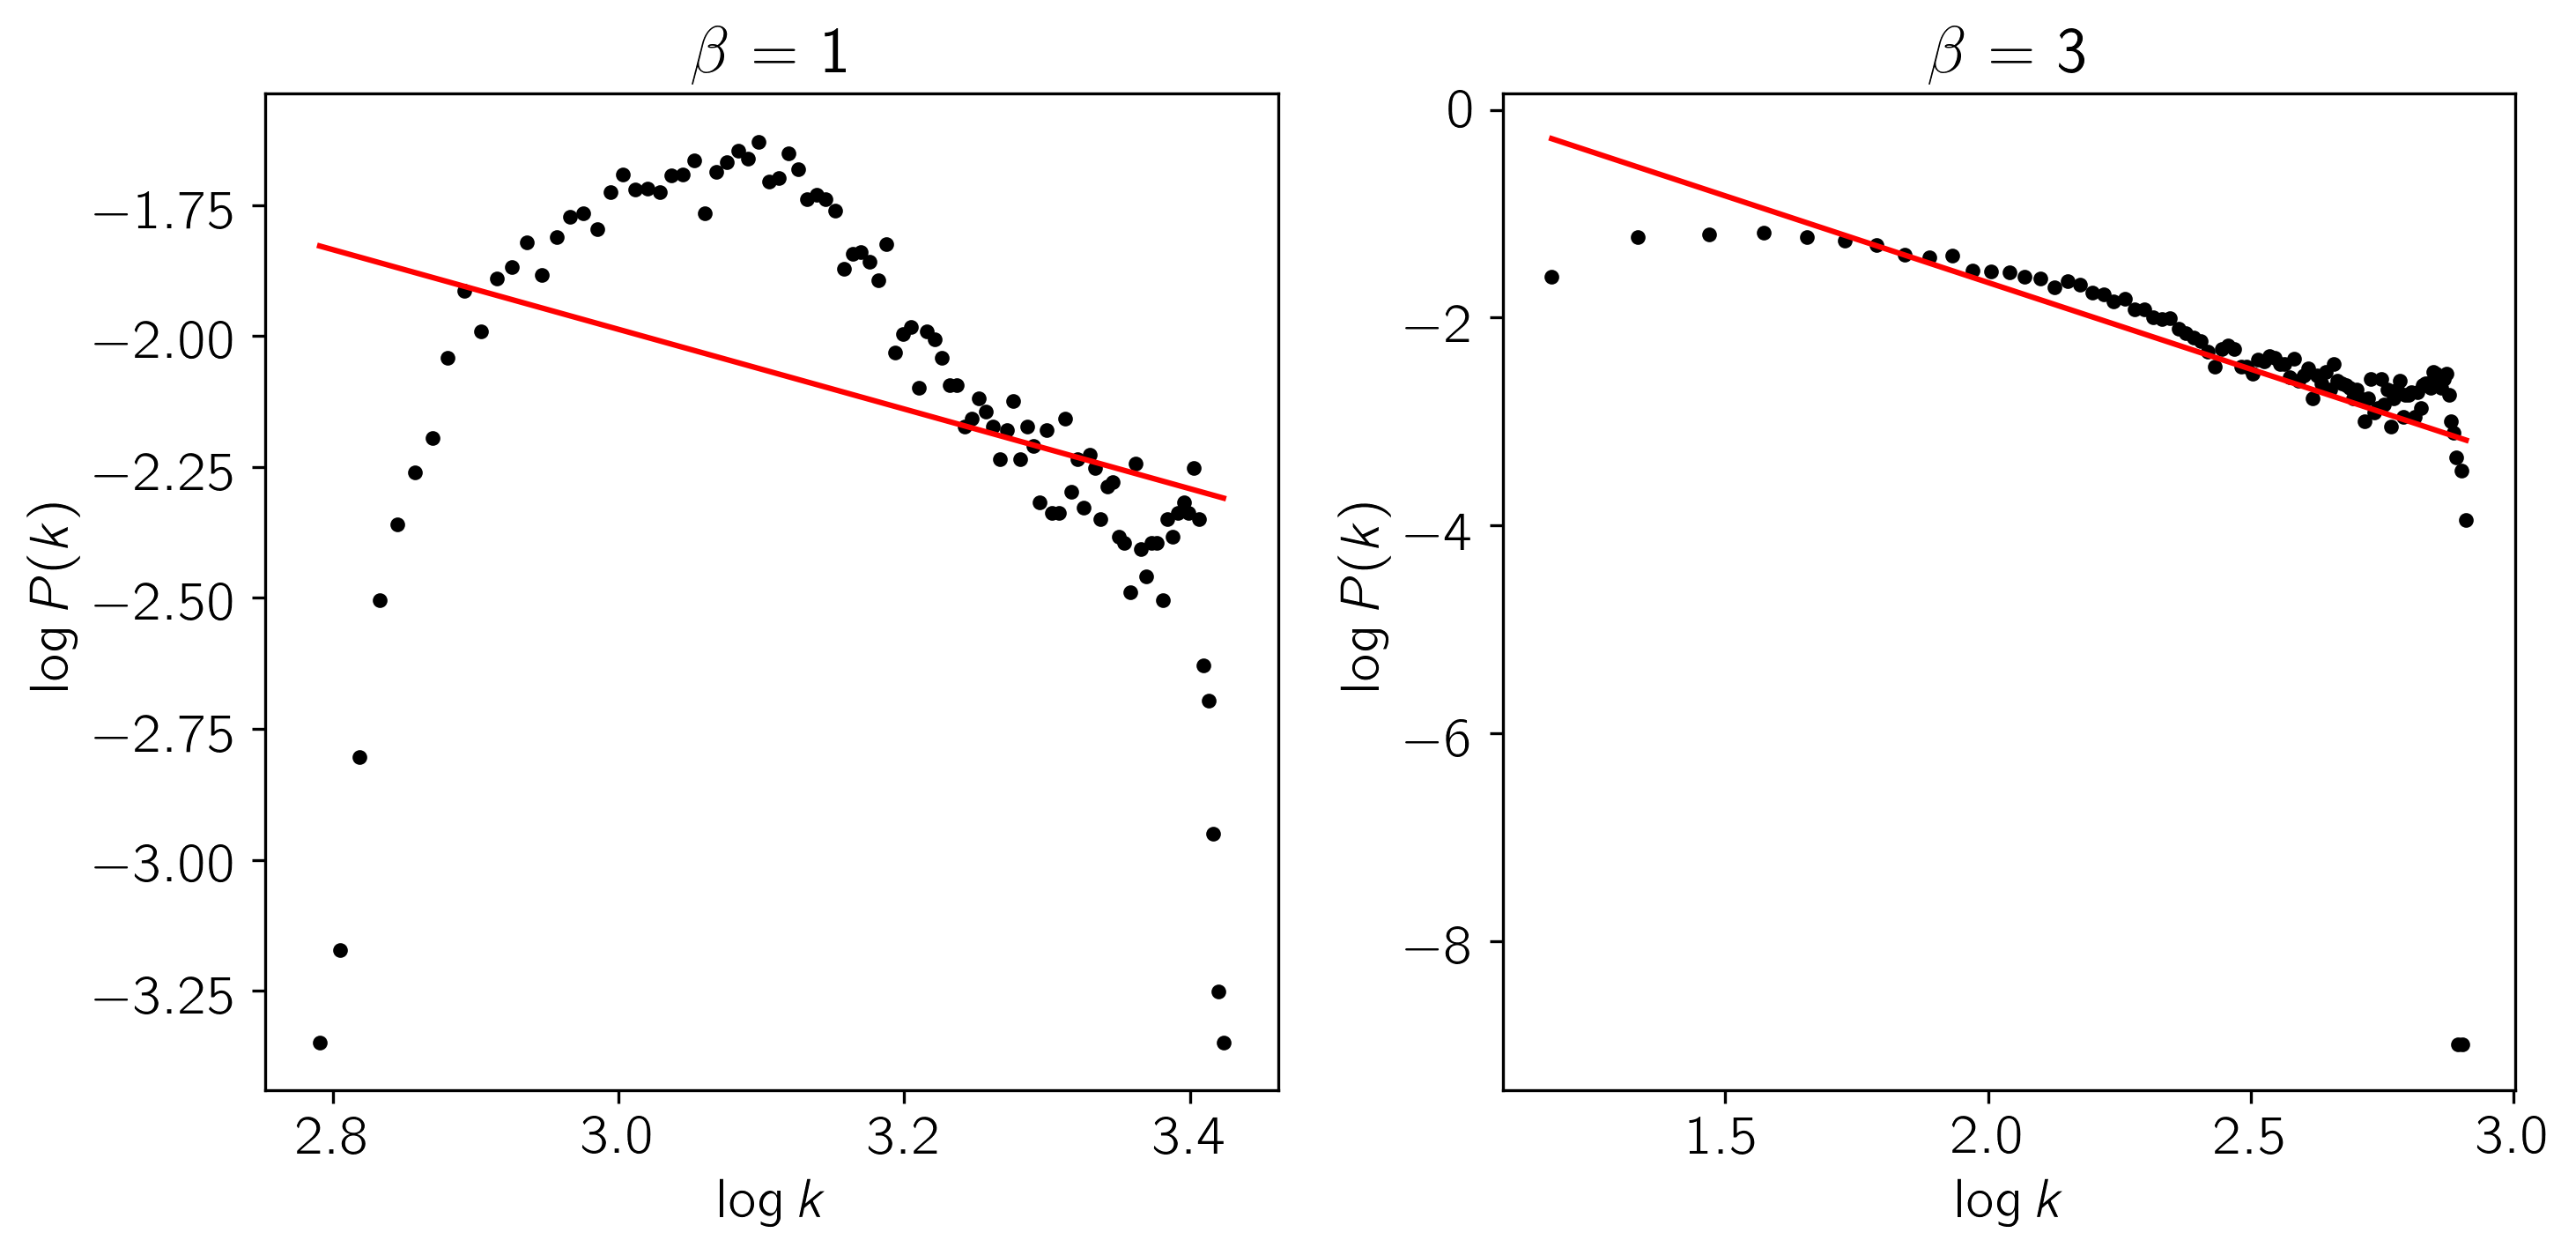
\includegraphics[clip,width=0.8\textwidth]{figures/figure2.png}
  \caption{Degree distribution of the network represented by $S$ (left) and $A$ (right).}
  \label{fig:beta}
\end{figure}

The resulting adjacency matrix $A$ represents a complete graph
$G=(V,E)$, with $|V| = 8\,928$ genes ($|E| = 39\,850\,128$ edges).

\subsection*{C. Identification of Co-expression Modules}

The adjacency matrix $A$ is transformed into an unweighted network
$\hat{A}$ applying the approach described
in~\cite{aoki2007approaches}. The cutoff value is set to $0.2$, 
based on the density of the network
combined with the decreasing number of nodes and edges with higher PCC
values. Thus keeping only the
connections above this threshold and removing any isolated nodes. The
resulting adjacency matrix $\hat{A}$ has $5\,810$ connected genes and
accounts for $614\,501$ edges.
\vspace{0.5cm}

After applying the HLC algorithm, a total of $4\,131$ genes are
distributed in $c = 5\,143$ overlapping modules of at least $3$
genes. Figure~\ref{fig:overlap} presents a histogram of the
overlapping percentage of these genes, measured as the proportion of
modules to which each gene belongs. The first bar of the histogram
represents the genes with zero overlap, corresponding to $28\%$ of the
total genes; the remaining $72\%$ represents the genes belonging to
more than one module.

%figure 3
\begin{figure}[htbp]
  \centering
    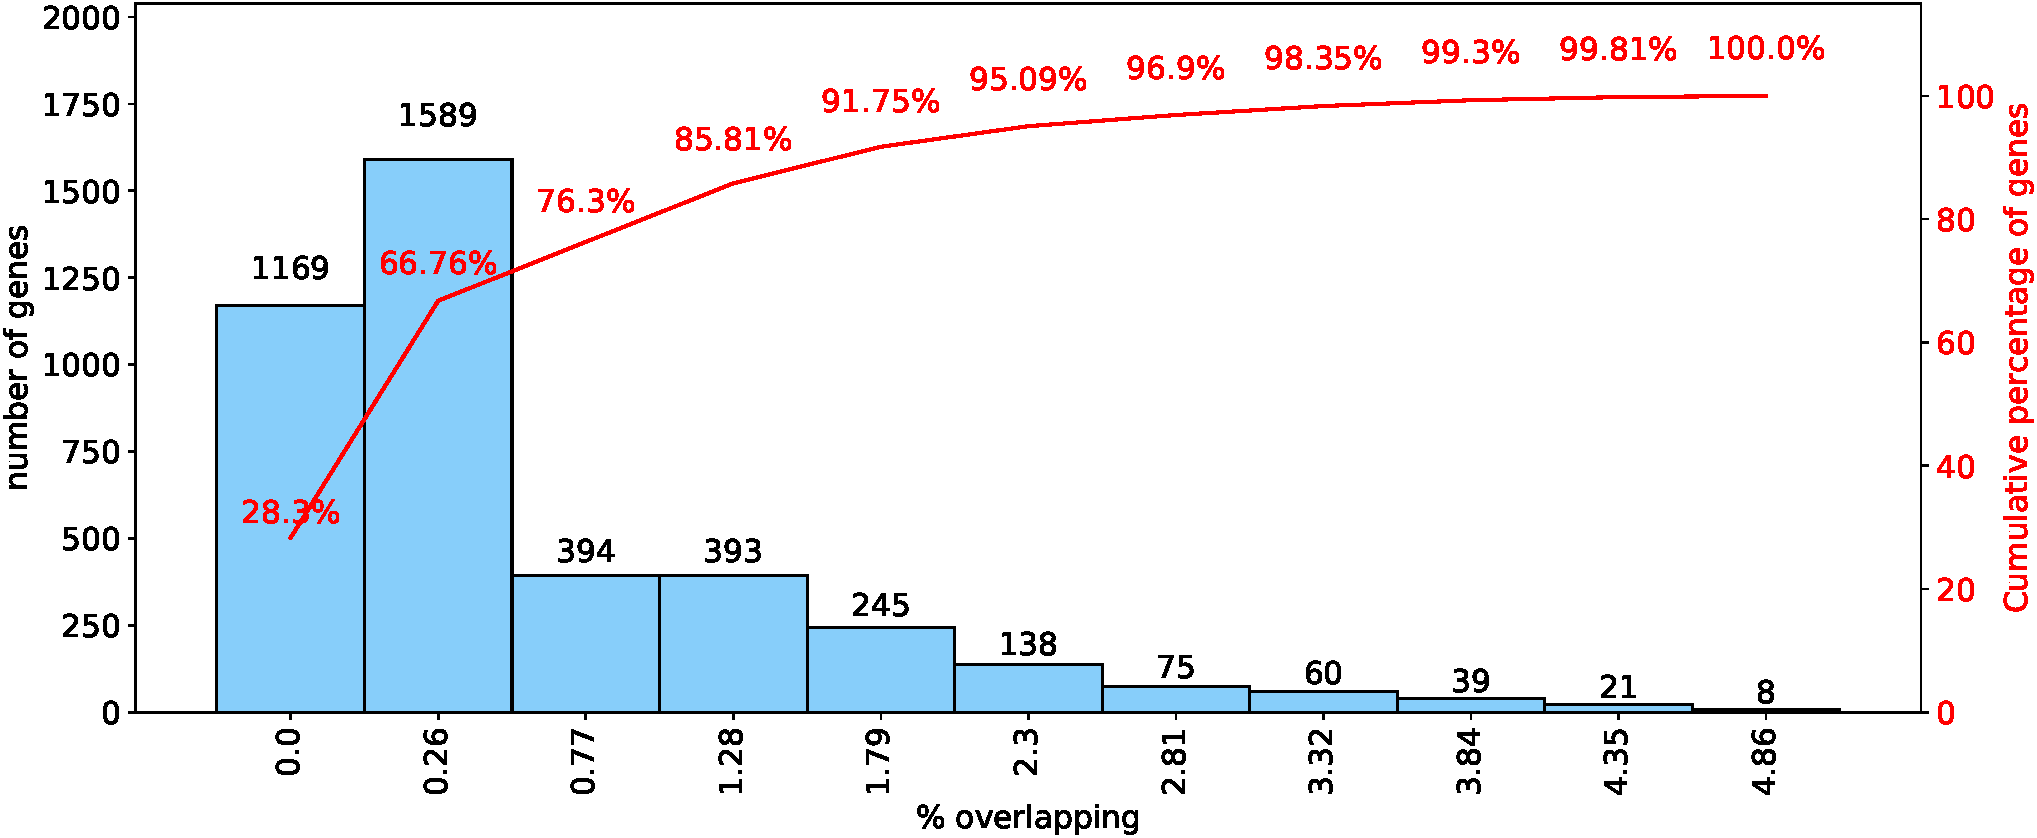
\includegraphics[clip,width=0.95\textwidth]{figures/figure3.pdf}
  \caption{Overlapping percentage of genes after applying HLC.}
  \label{fig:overlap}
\end{figure}

\subsection*{D. Detection of Modules Association to Phenotypic Traits}

The phenotypic traits under study are shoot $K$ content, root
biomass, and shoot biomass. Figure~\ref{fig:pdata} suggests that there
are significant differences in the values of these phenotypic traits
between stress and control conditions. This supports the working
hypothesis that these three variables represent tolerance-associated
traits in rice under salt stress.
\vspace{0.5cm}

%figure 4
\begin{figure}[htbp]
  \centering
    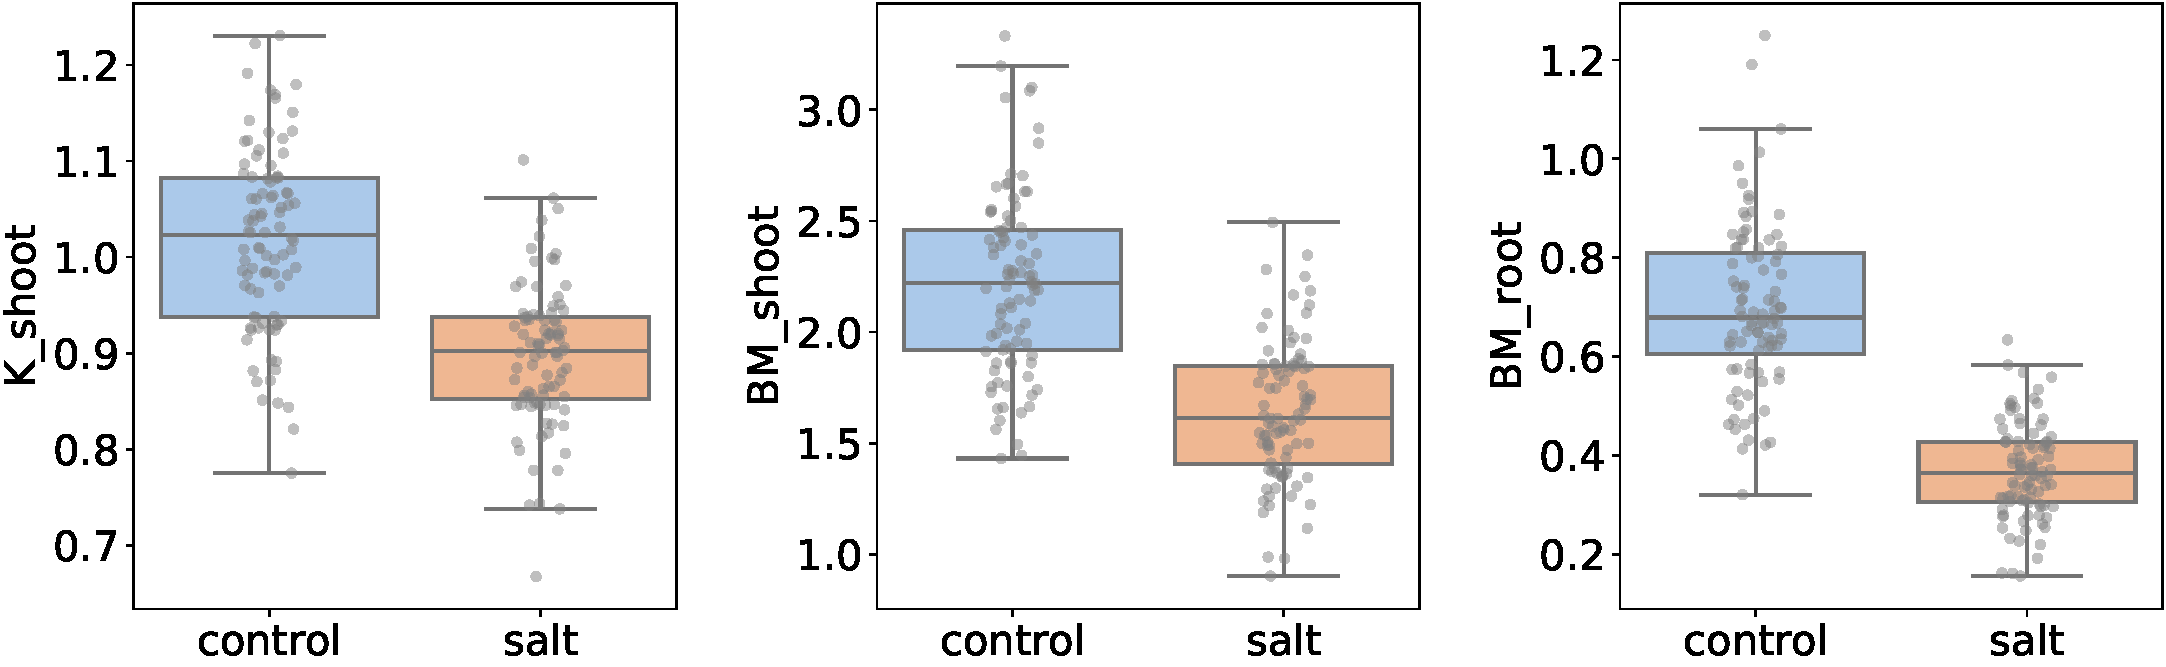
\includegraphics[clip,width=0.9\textwidth]{figures/figure4.pdf}
  \caption{Phenotipic traits distribution under control and salt stress.}
  \label{fig:pdata}
\end{figure}

Using the affiliation matrix $F$ derived from the HLC output and the
Log Fold Change matrix $L_1$, a matrix $M$ is built by computing the
eigengene for each of the $c = 5\,143$ modules. The LASSO technique is
applied by using each of the phenotypic traits as the outcome
variable, one at a time. As shown in Figure~\ref{fig:cross-val},
cross-validation is performed for each phenotypical trait in order to
select the corresponding regularization parameter $\lambda$ that
minimizes the mean-squared error.
\vspace{0.5cm}

%figure 5
\begin{figure}[htbp]
  \centering
    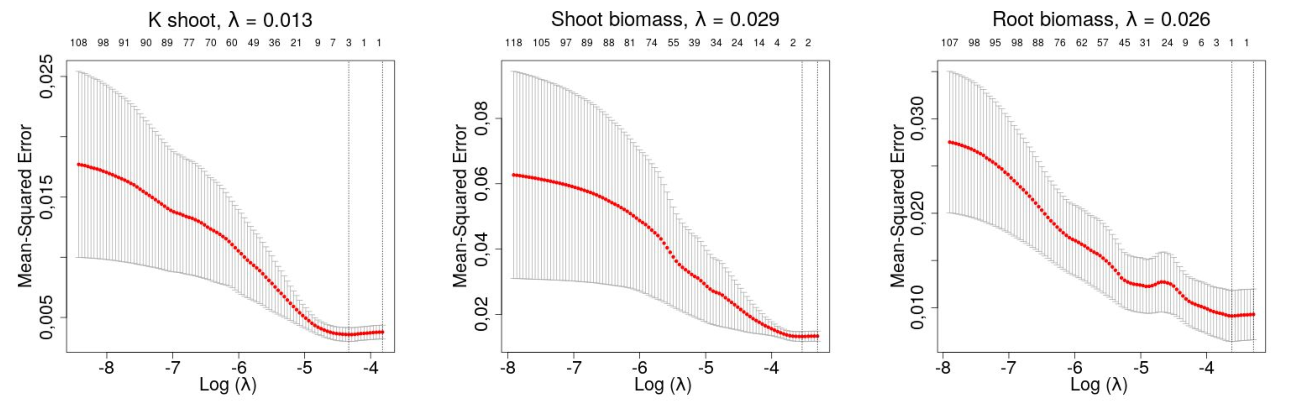
\includegraphics[clip,width=0.96\textwidth]{figures/figure5.pdf}
  \caption{Cross-validation of the LASSO regularization parameter
    $\lambda$, for each phenotypic trait.}
  \label{fig:cross-val}
\end{figure}

Finally, three LASSO models are adjusted by using the corresponding
$\lambda$ and phenotypical data with the eigengenes of matrix $M$. As
result, 6 modules are detected as relevant in the response to salt
stress in rice: 3 modules of 3 genes, each associated with shoot $K$
content; 2 modules of 3 genes associated with shoot biomass; and 1
module of 4 genes associated with root biomass (see
Figure~\ref{fig:final_genes}).

\subsection*{E. Gene Enrichment}

From the $19$ genes selected by LASSO, all but $3$ genes (the ones
associated to $K$ content), are also identified as deferentially
expressed ($|\ell_{ij}| \geq 2$) for at least one of the $92$
accessions. These genes are strong 
candidates target genes in rice.
%candidates as stress responsive genes to salt conditions in rice.
\vspace{0.5cm}

Figure~\ref{fig:final_genes} summarizes how from the initial
$n_0=57\,845$ genes, the proposed workflow identifies a reduced set of
$19$ genes. First, $48\,431$ genes are discarded after filtering the
normalized expression data $D_2$ and then $486$ additional genes are
discarded when filtering the Log Fold Change matrix $L_0$, to finally
arrive at $19$ genes, of which $16$ are differentially expressed.
\vspace{0.5cm}

% figure 6
\begin{figure}[htbp]
  \centering
    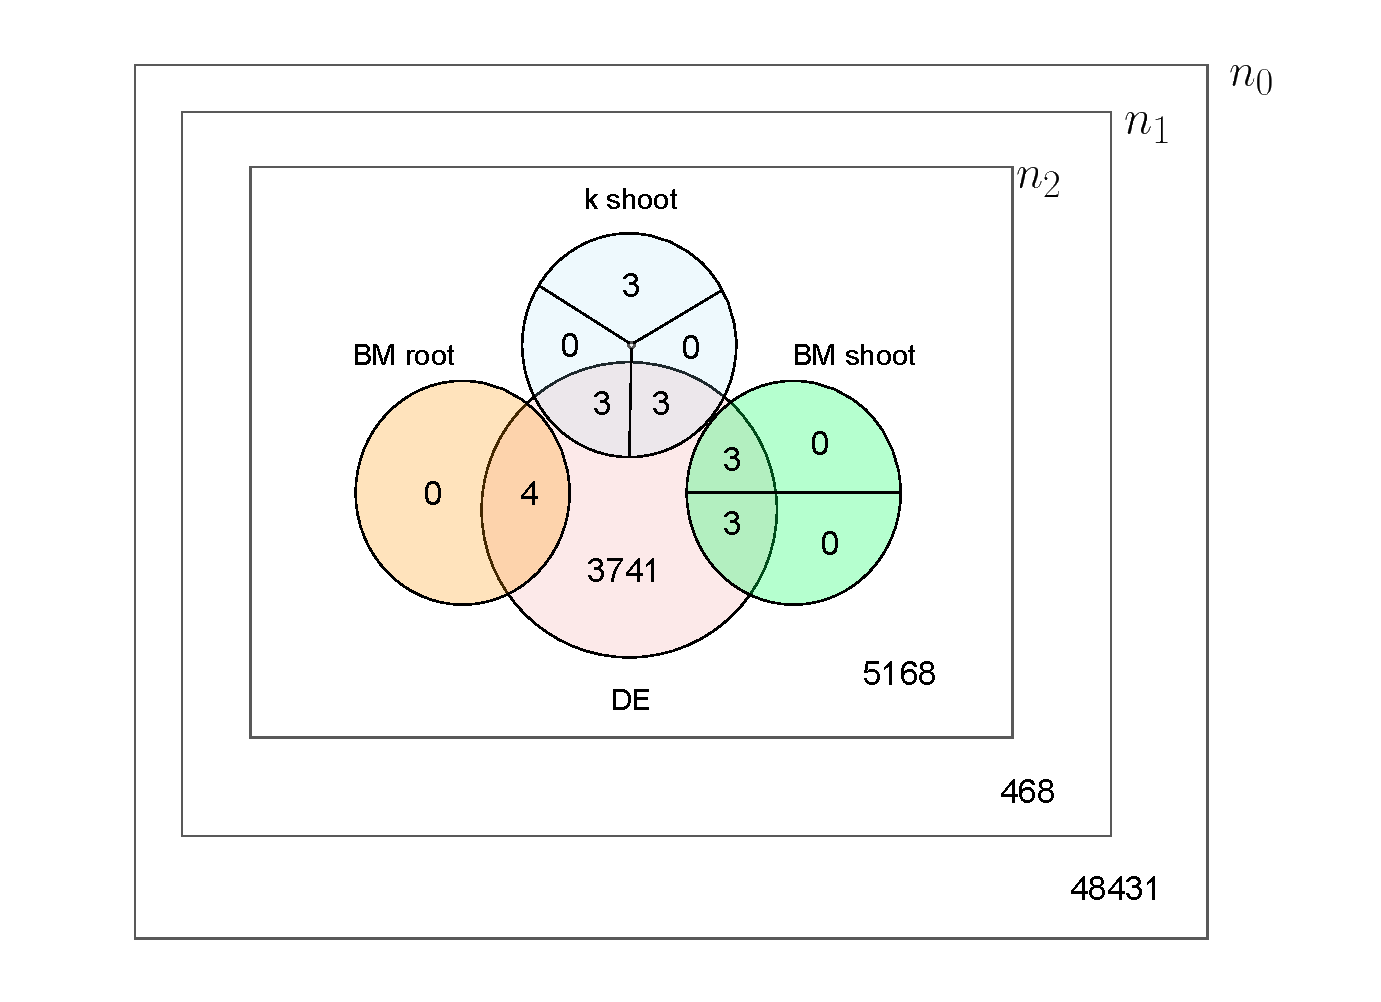
\includegraphics[clip,width=0.8\textwidth]{figures/figure6.pdf}
   \caption[Venn diagram for the case study in rice]%
   {Venn diagram representing the number of genes selected at
    different stages of the proposed workflow for the case study in
    rice.}
  \label{fig:final_genes}
\end{figure}

According to the Quickgo database, only $2$ of the $16$ differentially
expressed genes (both from the module related to shoot biomass) are
named and have an associated protein product: spermidine
hydroxycinnamoyltransferase 2 (SHT2) and lipoxygenase.
Figure~\ref{fig:3d} shows their corresponding 3D protein structures.
\vspace{0.5cm}

%figure 7
\begin{figure}[htbp]
  \centering
    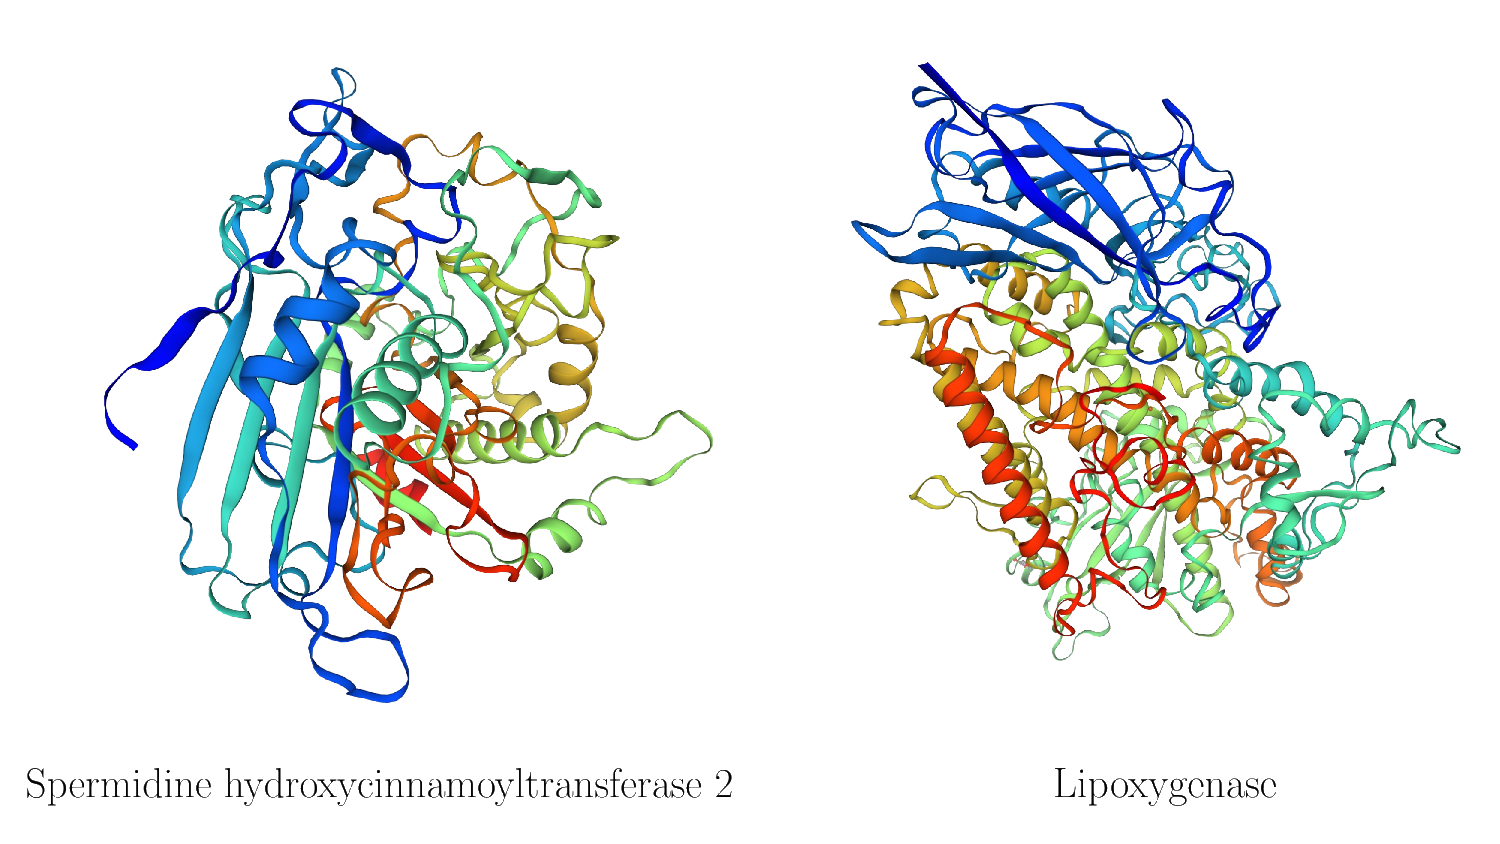
\includegraphics[clip,width=0.8\textwidth]{figures/figure7.pdf}
  \caption{3D protein structure of named genes selected by LASSO, borrowed from~\cite{szklarczyk2016string}.}
  \label{fig:3d}
\end{figure}

The Uniprot database~\cite{uniprot2018uniprot} reports, on the one
hand, that SHT2 contributes to the natural variation of
spermidine-based phenolamides in rice cultivars. On the other hand, it
is reported in~\cite{uniprot2018uniprot} that plant lipoxygenase may
be involved in a number of diverse aspects of plant physiology
including growth and development, pest resistance, and senescence or
responses to wounding. This protein is involved in the pathway
oxylipin biosynthesis, which is part of Lipid metabolism. Additionally,
previous studies
%
in~\cite{gupta2013plant,hou2015persimmon,mittova2002salt,peng2019novel,roychoudhury2011amelioration}
%
provide evidence of biological implications of sperimidine and
lipoxygenase in tolerance to salt stress in other plants or even in
rice cultivars.

As a conclusion, the results presented in this section suggest that
further studies are needed to elucidate the detailed biological
function of the remaining 14 genes that have not been named so far in
the literature.  They may have the potential to intervene in stress
responsive mechanisms to salt conditions in rice.


\section*{Related Work}

% related work: comparison between results here and results in literature
% trying to show why this paper is a contribution

(RELATED WORK GOES HERE)

\section*{Conclusion}

Based on previous work from other authors\cite{Kovacs2019}, the intrinsic
knowledge of existing protein-protein interaction networks let scientists
elucidate promising new interactions to explore. In this study, a
machine learning algorithm was fed with previously elucidated information
about the network, as well as results form a state-of-the-art edge
embedding technique. Even if the baseline of the handcrafted features
(A2, A3, L3) yields good results, boosting that information with the
vector embedding, which calculates vector representations of the network
structure improves the overall performance of each method on its own.

On both human interactomes (\emph{HI-II-14} and \emph{HI-TESTED}),
applying \texttt{XGBoost} with the metrics yield results with high
AUC for the link prediction problem, and therefore this study extends
previous work by other authors that only consider the predictive power
of the metrics alone. In this case, the importance of the handcrafted
features was very significant and stands out of the Node2Vec features.

On the rice interactome, PPI prediction obtained high AUC values when
only using the node embedding technique (AUC=0.93) and when only using
the handcrafted features based on protein neighborhood (AUC $\sim$ 0.88).
Even higher AUC results were achieved when the handcrafted features
and the vector representation information were combined (AUC $\sim$ 0.98).

Importance values for the A3 method stand out less from the node embedding
information than in A2 and L3. However, handcrafted features are more
important for the prediction of the human than in the rice interactome. 

With this study, a framework for link prediction on protein-protein
interactions is presented and validated against the available information
on rice and human interactomes. However, it might be easily extended
to other organisms or even to other graphs not necessarily related
to biology, because the only required information is the network connectivity.
Satisfactory results might be expected when the framework is applied
to networks with a dense adjacency matrix, since calculations of L3
and Node2Vec rely on network exploration for an arbitrary node and
its degree.


%\subsection*{Sub-heading for section}
%Text for this sub-heading\ldots
%\subsubsection*{Sub-sub heading for section}
%Text for this sub-sub-heading\ldots
%\paragraph*{Sub-sub-sub heading for section}
%Text for this sub-sub-sub-heading\ldots

%%%%%%%%%%%%%%%%%%%%%%%%%%%%%%%%%%%%%%%%%%%%%%
%%                                          %%
%% Backmatter begins here                   %%
%%                                          %%
%%%%%%%%%%%%%%%%%%%%%%%%%%%%%%%%%%%%%%%%%%%%%%

\begin{backmatter}

\section*{Acknowledgements}%% if any
Not applicable

\section*{Funding}%% if any
This work was funded by the OMICAS program: Optimización Multiescala In-silico de
Cultivos Agrícolas Sostenibles (Infraestructura y Validación en Arroz y Caña de Azúcar),
anchored at the Pontificia Universidad Javeriana in Cali and funded within the Colombian
Scientific Ecosystem by The World Bank, the Colombian Ministry of Science, Technology and
Innovation, the Colombian Ministry of Education and the Colombian Ministry of Industry 
and Turism, and ICETEX, under GRANT ID: FP44842-217-2018.

\section*{Abbreviations}%% if any
\textbf{HLC:} Hierarchical Link Clustering\\
\textbf{LASSO:} Least Absolute Shrinkage Selector Operator\\
\textbf{PCC:} Pearson Correlation Coefficient\\
\textbf{RNA-seq:} RNA sequencing\\
\textbf{SHT2:} Spermidine hydroxycinnamoyltransferase 2\\
\textbf{WGCNA:} Weighted Gene Co-expression Network Analysis

\section*{Availability of data and materials}%% if any
The datasets analysed during the current study are publicy available. They can be found in the following locations:
\begin{itemize}
\item RNA-seq data of salt stress in rice is available on the GEO (GSE98455).
\item Phenotypic data of salt stress in rice is a subset of the supplementary file 1 included in ~\cite{campbell2017allelic}.
\end{itemize}

\section*{Ethics approval and consent to participate}%% if any
Not applicable

\section*{Competing interests}
The authors declare that they have no competing interests.

\section*{Consent for publication}%% if any
Not applicable

\section*{Authors' contributions}
J.F. and C.R. proposed the original idea. 
J.F. provide advice on algorithms concepts and implementation.
C.R. structured the methodology and performed the analysis. 
C.R., J.F., and H.C.R. wrote the manuscript.
All authors read and approved the final manuscript.


%
%%%%%%%%%%%%%%%%%%%%%%%%%%%%%%%%%%%%%%%%%%%%%%%%%%%%%%%%%%%%%
%%                  The Bibliography                       %%
%%                                                         %%
%%  Bmc_mathpys.bst  will be used to                       %%
%%  create a .BBL file for submission.                     %%
%%  After submission of the .TEX file,                     %%
%%  you will be prompted to submit your .BBL file.         %%
%%                                                         %%
%%                                                         %%
%%  Note that the displayed Bibliography will not          %%
%%  necessarily be rendered by Latex exactly as specified  %%
%%  in the online Instructions for Authors.                %%
%%                                                         %%
%%%%%%%%%%%%%%%%%%%%%%%%%%%%%%%%%%%%%%%%%%%%%%%%%%%%%%%%%%%%%

% if your bibliography is in bibtex format, use those commands:
\bibliographystyle{bmc-mathphys} % Style BST file (bmc-mathphys, vancouver, spbasic).
\bibliography{bmc_article}      % Bibliography file (usually '*.bib' )
% for author-year bibliography (bmc-mathphys or spbasic)
% a) write to bib file (bmc-mathphys only)
% @settings{label, options="nameyear"}
% b) uncomment next line
%\nocite{label}

% or include bibliography directly:
% \begin{thebibliography}
% \bibitem{b1}
% \end{thebibliography}

%%%%%%%%%%%%%%%%%%%%%%%%%%%%%%%%%%%
%%                               %%
%% Figures                       %%
%%                               %%
%% NB: this is for captions and  %%
%% Titles. All graphics must be  %%
%% submitted separately and NOT  %%
%% included in the Tex document  %%
%%                               %%
%%%%%%%%%%%%%%%%%%%%%%%%%%%%%%%%%%%

%%
%% Do not use \listoffigures as most will included as separate files

%\section*{Figures}
%  \begin{figure}[h!]
%  \caption{Sample figure title}
%\end{figure}
%
%\begin{figure}[h!]
%  \caption{Sample figure title}
%\end{figure}

%%%%%%%%%%%%%%%%%%%%%%%%%%%%%%%%%%%
%%                               %%
%% Tables                        %%
%%                               %%
%%%%%%%%%%%%%%%%%%%%%%%%%%%%%%%%%%%

%% Use of \listoftables is discouraged.
%%
%\section*{Tables}
%\begin{table}[h!]
%\caption{Sample table title. This is where the description of the table should go}
%  \begin{tabular}{cccc}
%    \hline
%    & B1  &B2   & B3\\ \hline
%    A1 & 0.1 & 0.2 & 0.3\\
%    A2 & ... & ..  & .\\
%    A3 & ..  & .   & .\\ \hline
%  \end{tabular}
%\end{table}

%%%%%%%%%%%%%%%%%%%%%%%%%%%%%%%%%%%
%%                               %%
%% Additional Files              %%
%%                               %%
%%%%%%%%%%%%%%%%%%%%%%%%%%%%%%%%%%%


\section*{Appendix}

\subsection*{Node2Vec Parameters}

For all experiments, the following parameters hold:
\begin{itemize}
\item For the (\texttt{p=1}, \texttt{q=1})
\item (\texttt{dimensions=16, workers=4})
\item (\texttt{walk\_length=5}, \texttt{num\_walks=300}, \texttt{window=5})
\item (\texttt{min\_count=1}, \texttt{batch\_words=4})
\item (\texttt{EdgeEmbedding=EdgeHadamardEmbedder})
\end{itemize}

\subsection*{XGBoost parameters}
\begin{itemize}
\item \texttt{max\_depth=3}
\item \texttt{colsample\_bytree=0.6}
\item \texttt{eval\_metric='auc'}
\end{itemize}



\subsection*{Supplementary Figures for Human Interactome}

\begin{figure}[h]
\noindent \begin{centering}
\caption{\label{HI1}\emph{HI-II-14} results for \texttt{Node2Vec} with A2
feature}
\par\end{centering}
\noindent \raggedleft{}\includegraphics[width=0.48\columnwidth]{figures/Human/ROC\lyxdot A2}\includegraphics[width=0.48\columnwidth]{figures/Human/CM\lyxdot A2}
\end{figure}

\begin{figure}[h]
\noindent \begin{centering}
\caption{\label{HI2}\emph{HI-II-14} results for \texttt{Node2Vec} with A3
feature}
\par\end{centering}
\noindent \raggedleft{}\includegraphics[width=0.48\columnwidth]{figures/Human/ROC\lyxdot A3}\includegraphics[width=0.48\columnwidth]{figures/Human/CM\lyxdot A3}
\end{figure}

\begin{figure}[h]
\noindent \begin{centering}
\caption{\label{HI3}\emph{HI-II-14} results for \texttt{Node2Vec} with L3
feature}
\par\end{centering}
\noindent \raggedleft{}\includegraphics[width=0.48\columnwidth]{figures/Human/ROC\lyxdot L3}\includegraphics[width=0.48\columnwidth]{figures/Human/CM\lyxdot L3}
\end{figure}

\begin{figure}[h]
\noindent \begin{centering}
\caption{\label{HI1-1}\emph{HI-TESTED} results for \texttt{Node2Vec} with
A2 feature}
\par\end{centering}
\noindent \raggedleft{}\includegraphics[width=0.48\columnwidth]{figures/Human/ROC\lyxdot A2\lyxdot 2}\includegraphics[width=0.48\columnwidth]{figures/Human/CM\lyxdot A2\lyxdot 2}
\end{figure}

\begin{figure}[h]
\noindent \begin{centering}
\caption{\label{HI2-1}\emph{HI-TESTED} results for \texttt{Node2Vec} with
A3 feature}
\par\end{centering}
\noindent \raggedleft{}\includegraphics[width=0.48\columnwidth]{figures/Human/ROC\lyxdot A3\lyxdot 2}\includegraphics[width=0.48\columnwidth]{figures/Human/CM\lyxdot A3\lyxdot 2}
\end{figure}

\begin{figure}[h]
\noindent \begin{centering}
\caption{\label{HI3-1}\emph{HI-TESTED} results for \texttt{Node2Vec} with
L3 feature}
\par\end{centering}
\noindent \raggedleft{}\includegraphics[width=0.48\columnwidth]{figures/Human/ROC\lyxdot L3\lyxdot 2}\includegraphics[width=0.48\columnwidth]{figures/Human/CM\lyxdot L3\lyxdot 2}
\end{figure}

\begin{figure}[h]
\noindent \begin{centering}
\caption{\label{F8-importance-H2}Importance gain plots for \emph{HI-TESTED}}
\par\end{centering}
\begin{centering}
\includegraphics[width=0.7\columnwidth]{figures/Human/Imp\lyxdot A2\lyxdot 2}
\par\end{centering}
\begin{centering}
\includegraphics[width=0.7\columnwidth]{figures/Human/Imp\lyxdot A3\lyxdot 2}
\par\end{centering}
\centering{}\includegraphics[width=0.7\columnwidth]{figures/Human/Imp\lyxdot L3\lyxdot 2}
\end{figure}


\subsection*{Supplementary Figures for Rice Interactome}

\begin{figure}[h]
\noindent \begin{centering}
\caption{\label{F2}Results for \texttt{Node2Vec} with A2 feature}
\par\end{centering}
\noindent \raggedleft{}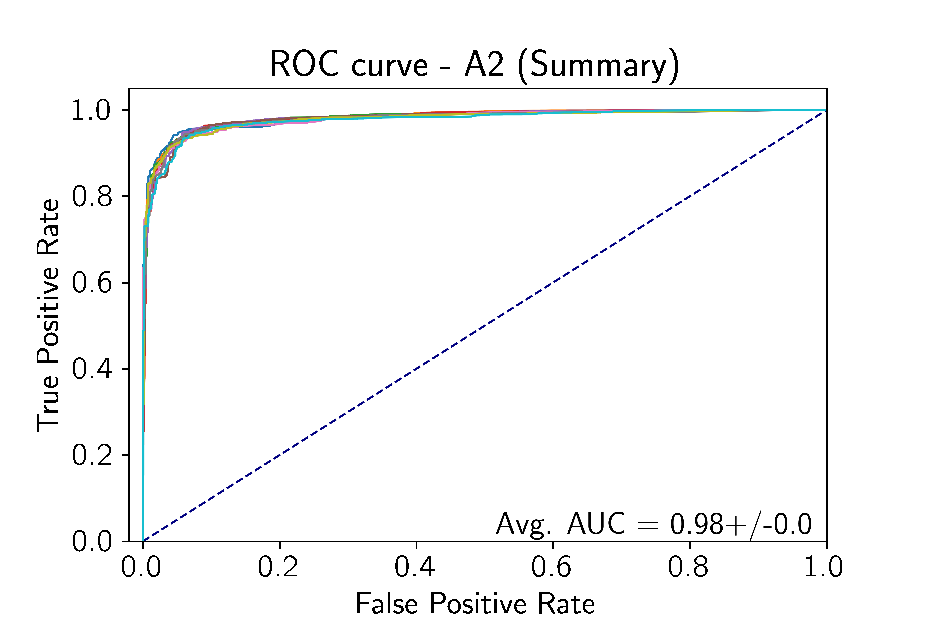
\includegraphics[width=0.48\columnwidth]{figures/ML_Metric/ROCA2_SUMMARY}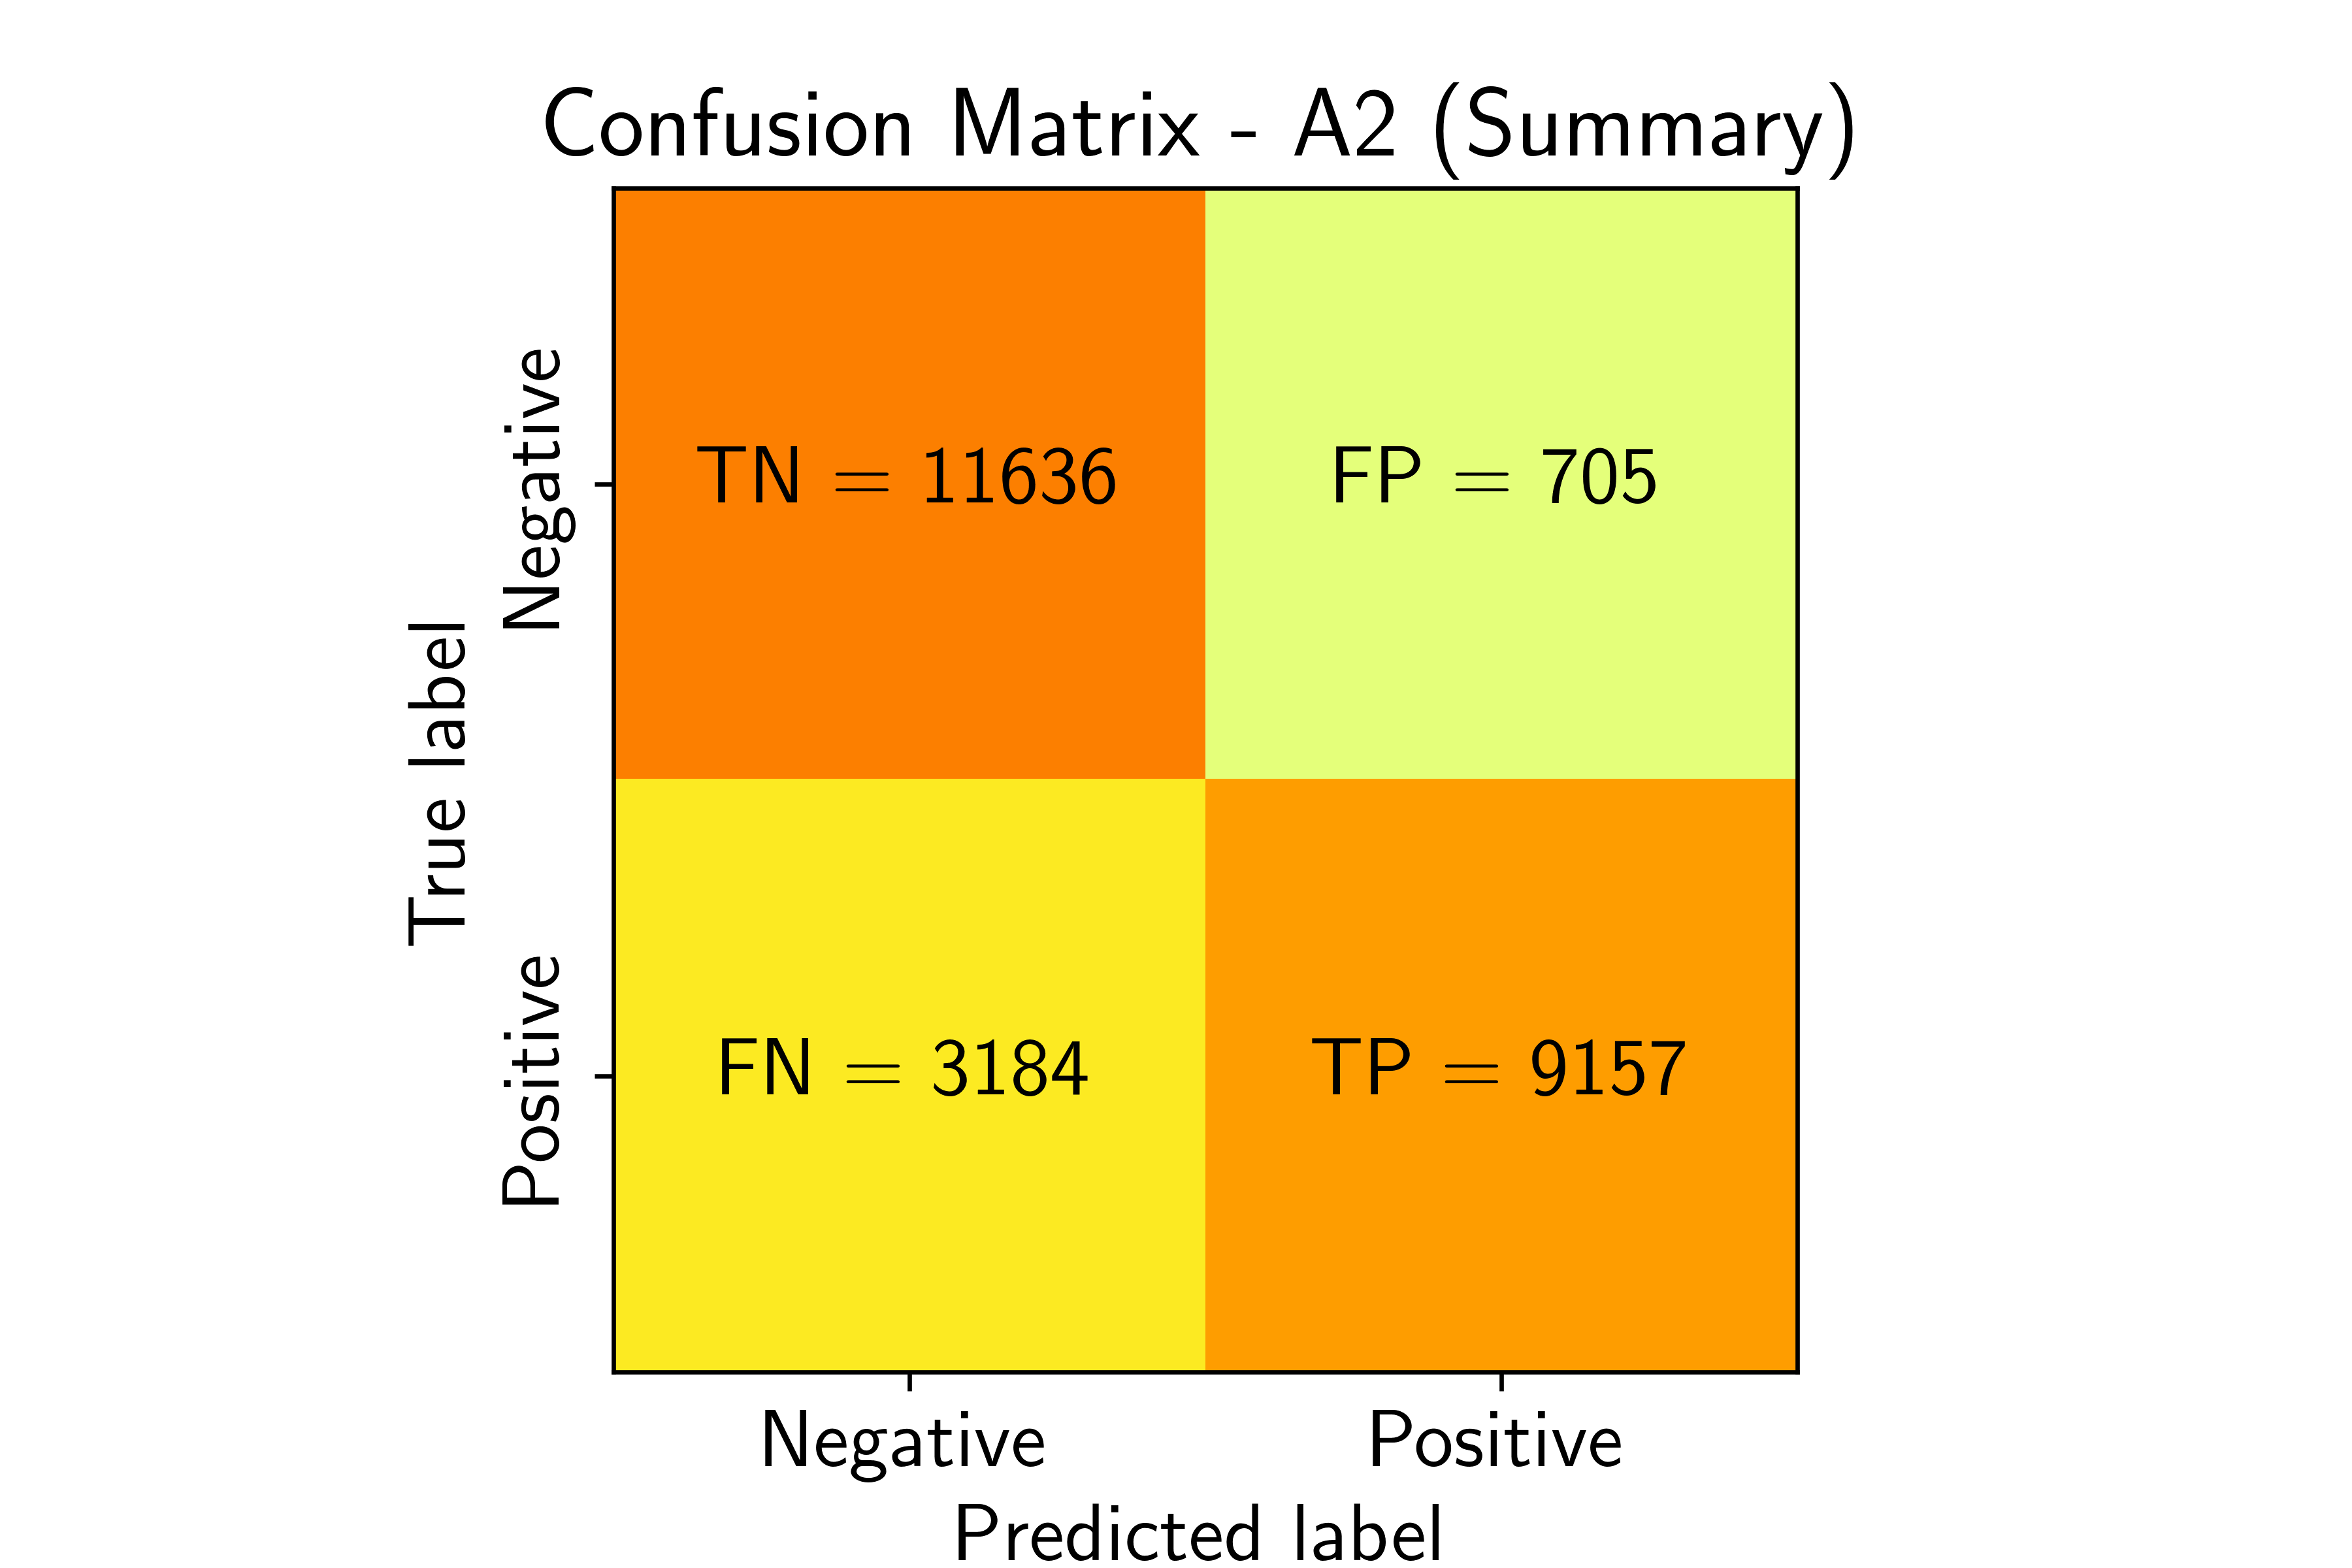
\includegraphics[width=0.48\columnwidth]{figures/ML_Metric/CMA2_SUMMARY}
\end{figure}

\begin{figure}[h]
\noindent \begin{centering}
\caption{\label{F3}Results for \texttt{Node2Vec} with A3 feature}
\par\end{centering}
\noindent \raggedleft{}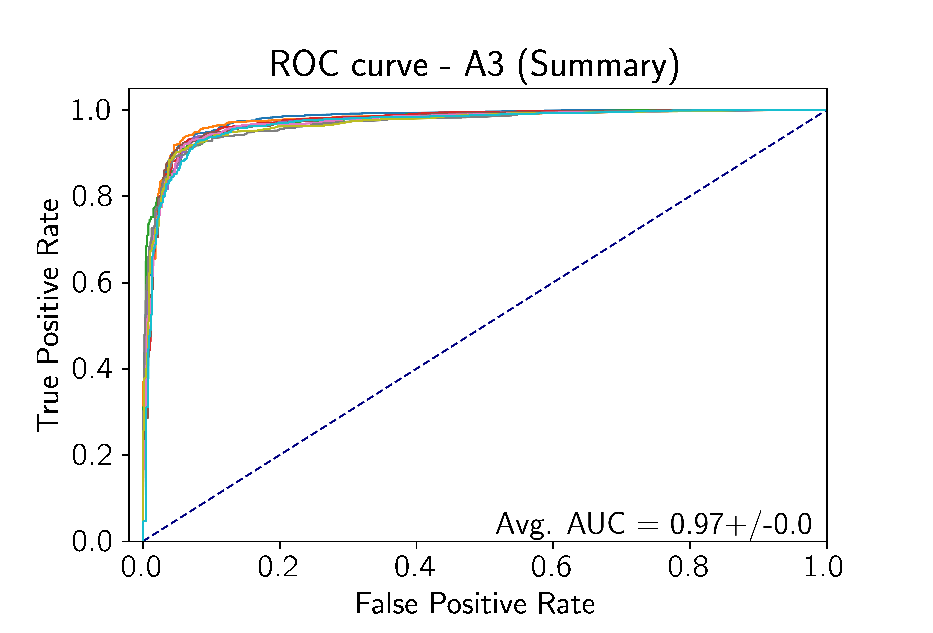
\includegraphics[width=0.48\columnwidth]{figures/ML_Metric/ROCA3_SUMMARY}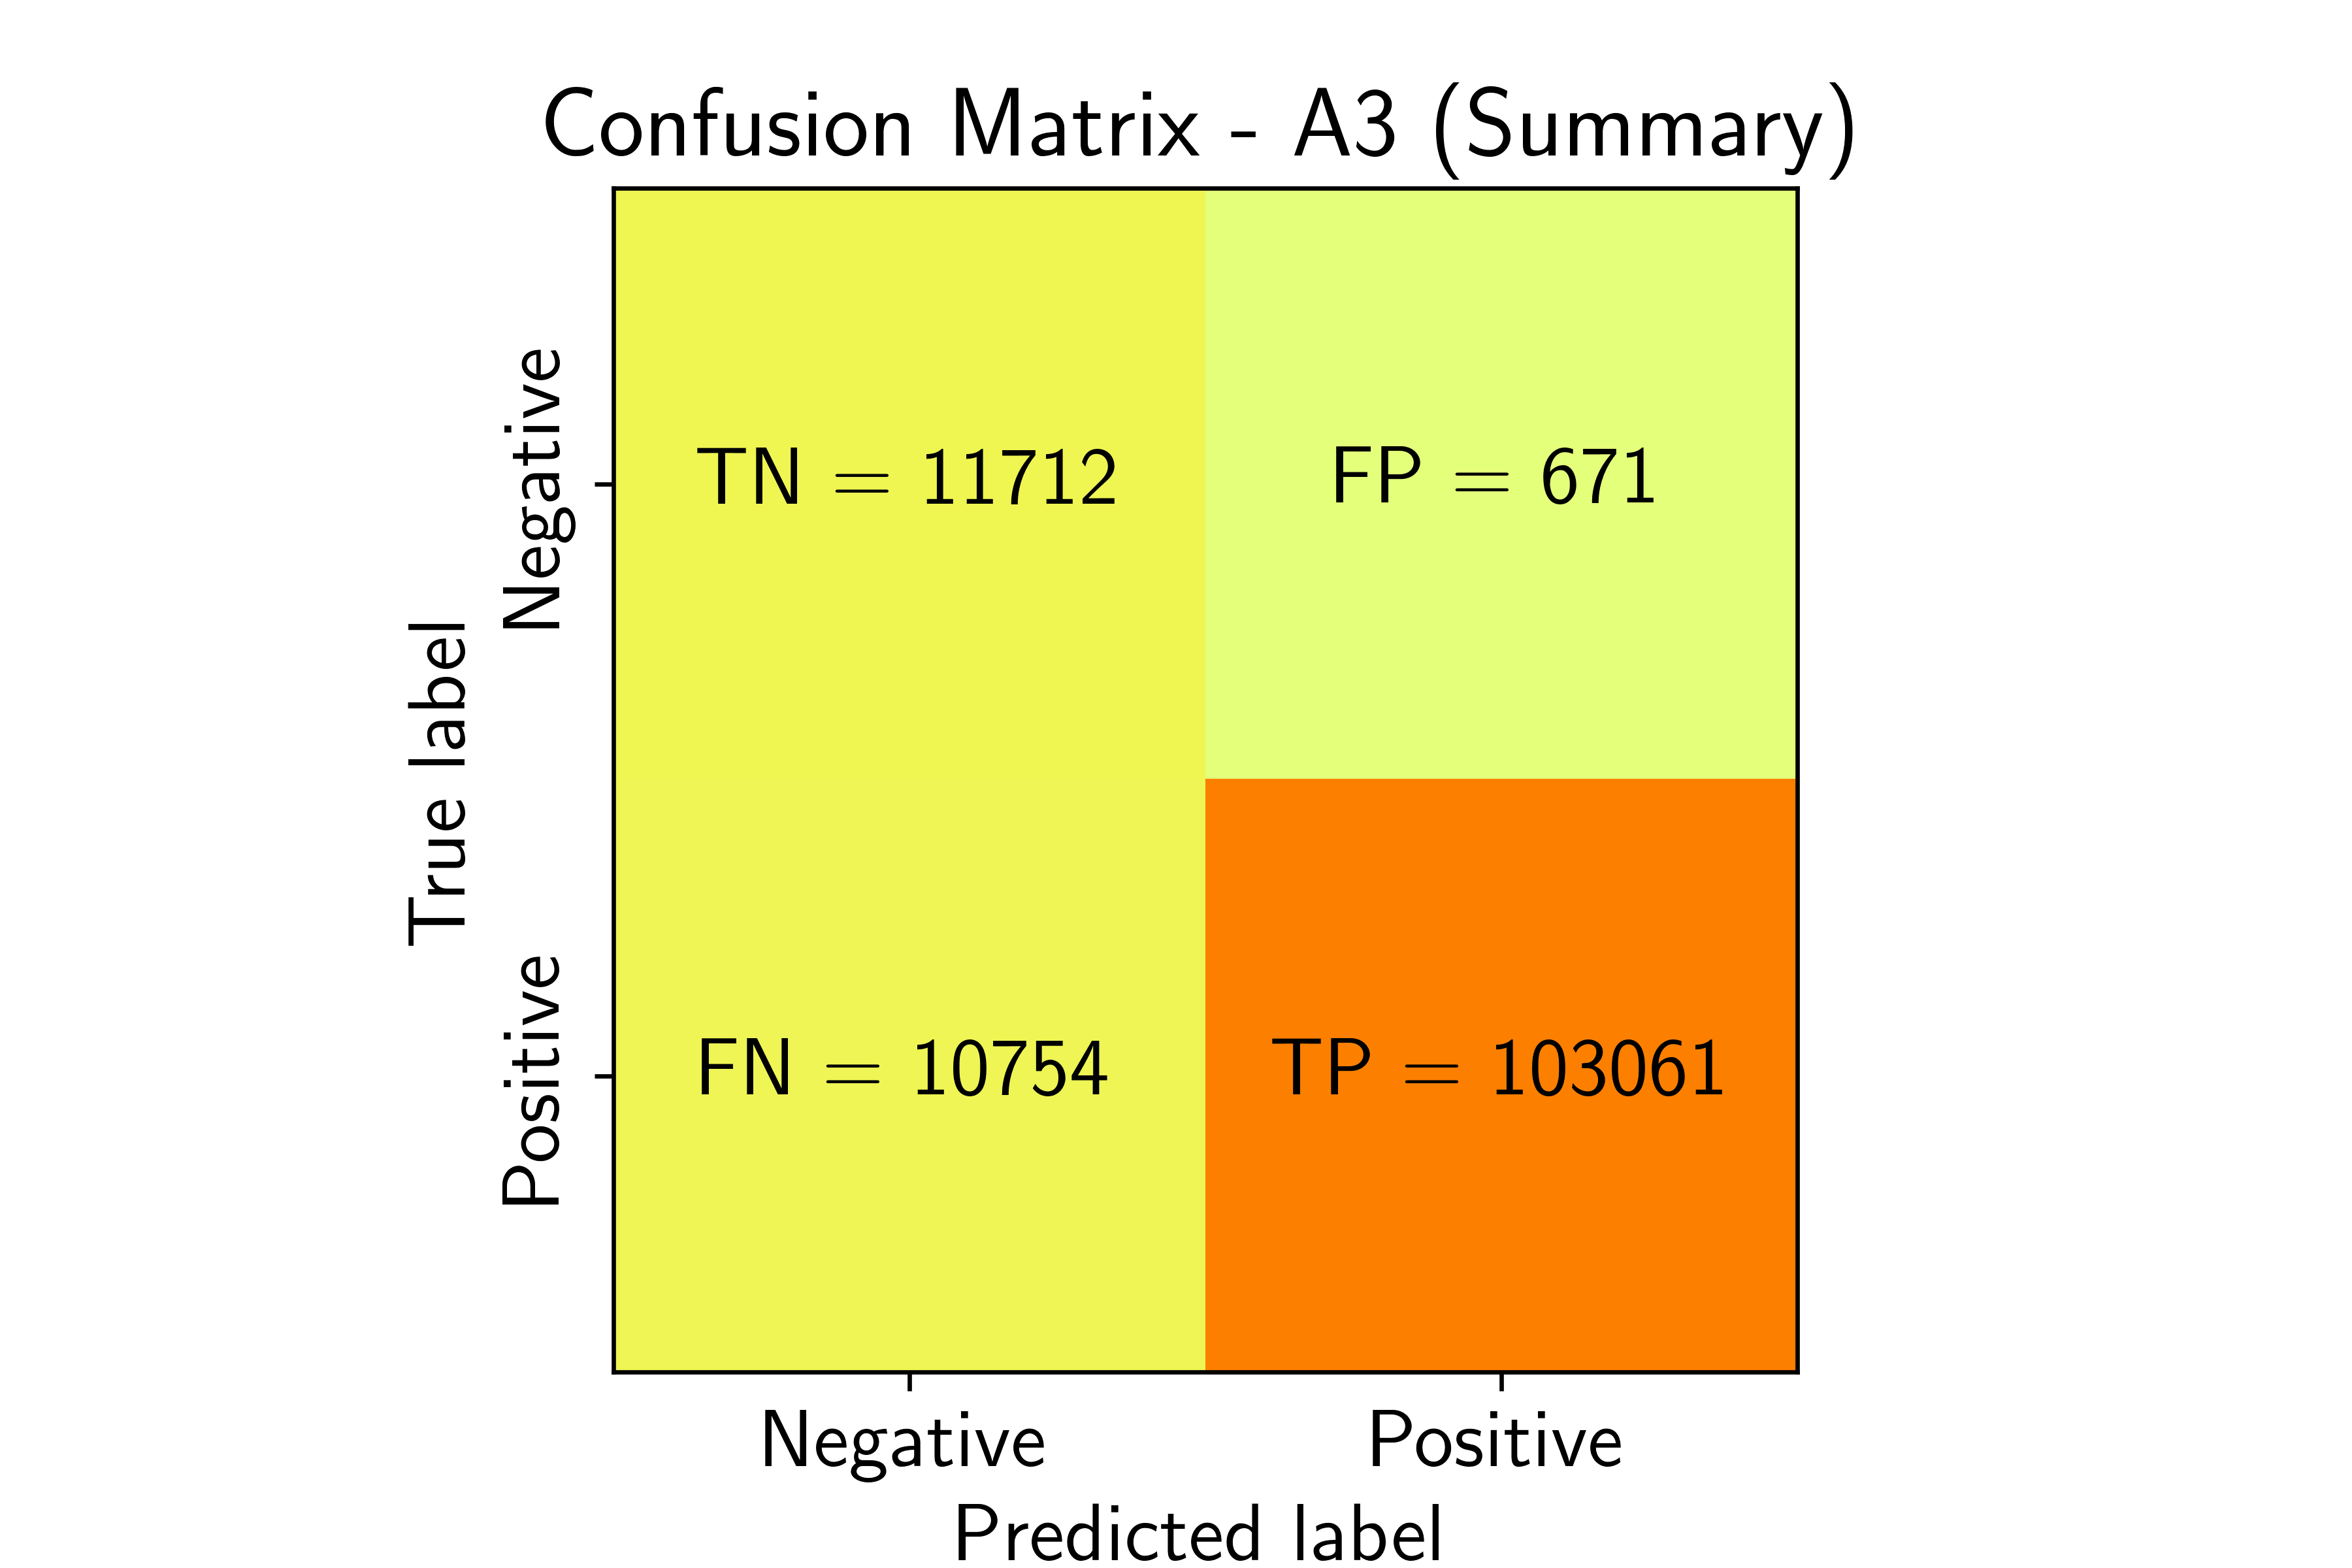
\includegraphics[width=0.48\columnwidth]{figures/ML_Metric/CMA3_SUMMARY}
\end{figure}

\begin{figure}[h]
\noindent \begin{centering}
\caption{\label{F5}Results for A2 feature only}
\par\end{centering}
\noindent \raggedleft{}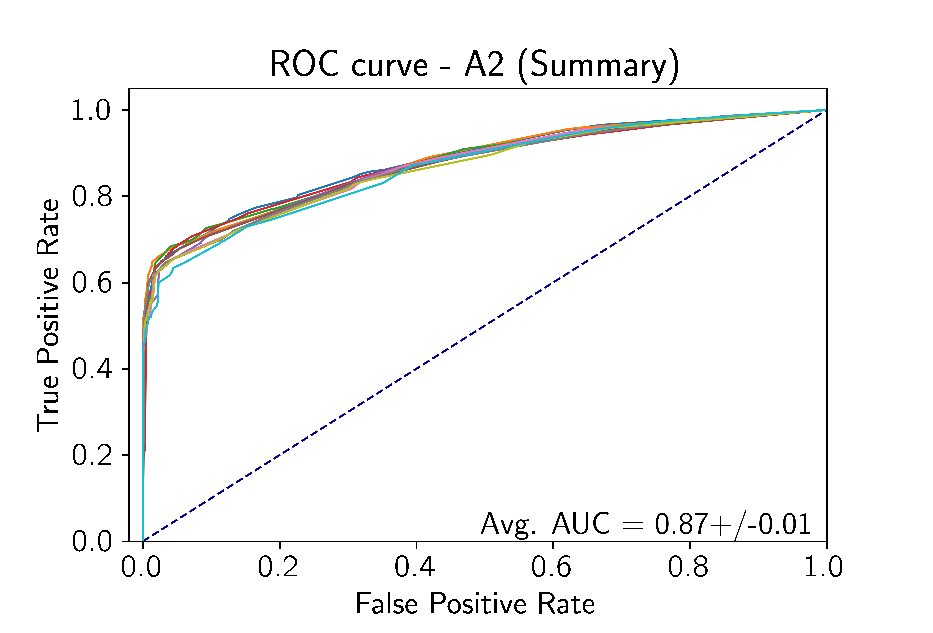
\includegraphics[width=0.48\columnwidth]{figures/Only_Metric/ROConlyA2_SUMMARY}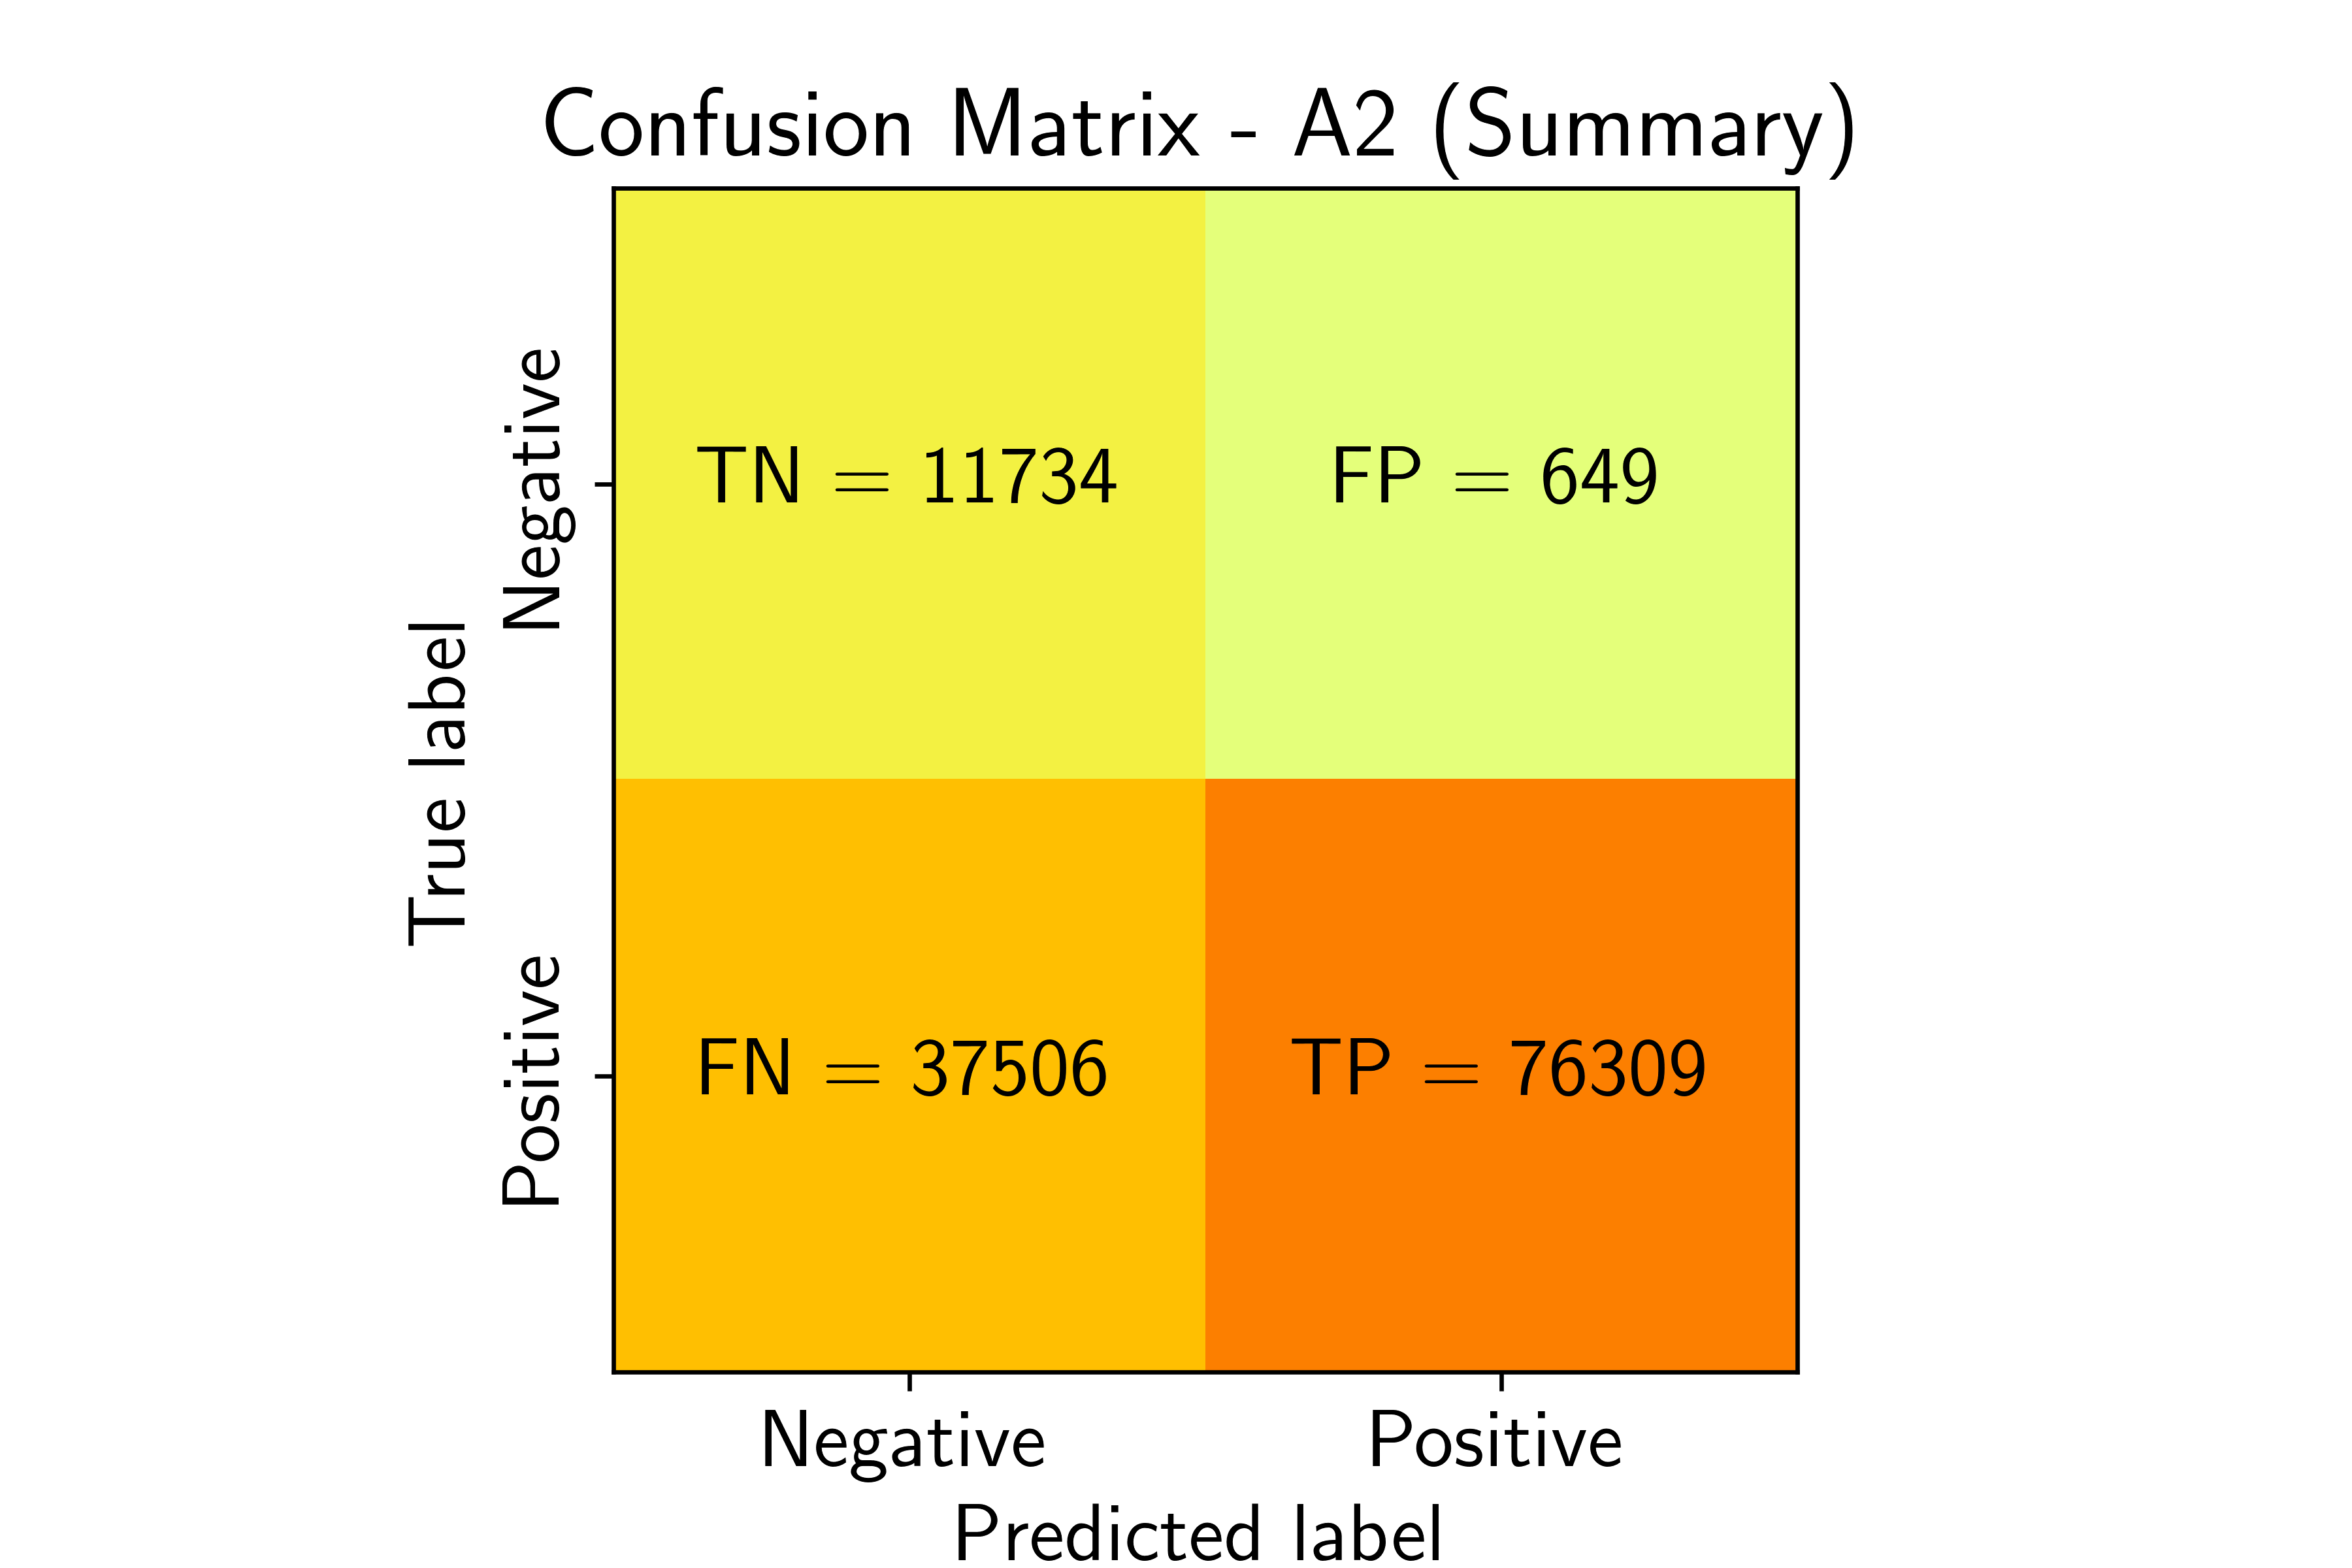
\includegraphics[width=0.48\columnwidth]{figures/Only_Metric/CMonlyA2_SUMMARY}
\end{figure}

\begin{figure}[h]
\noindent \begin{centering}
\caption{\label{F6}Results for A3 feature alone}
\par\end{centering}
\noindent \raggedleft{}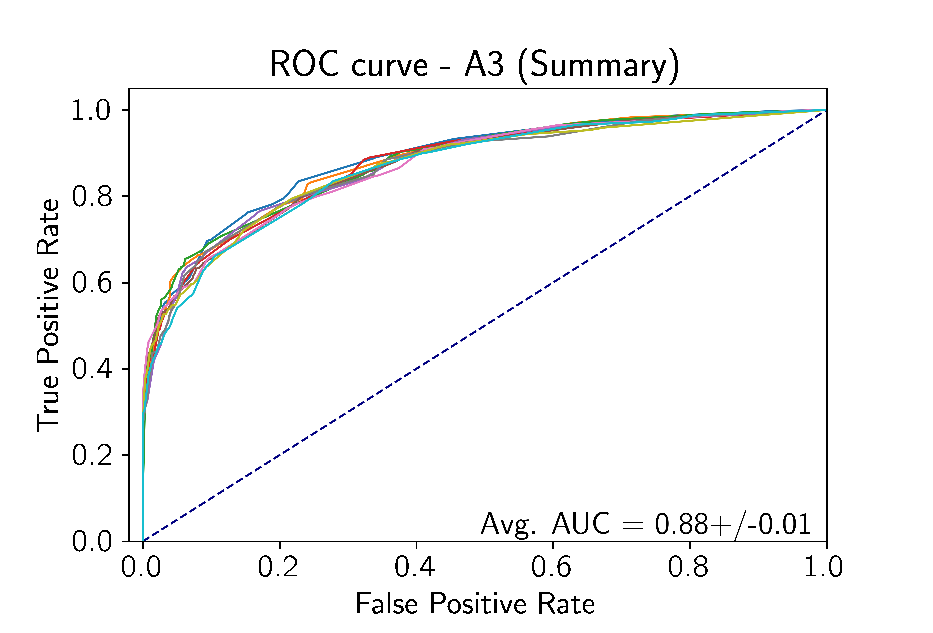
\includegraphics[width=0.48\columnwidth]{figures/Only_Metric/ROConlyA3_SUMMARY}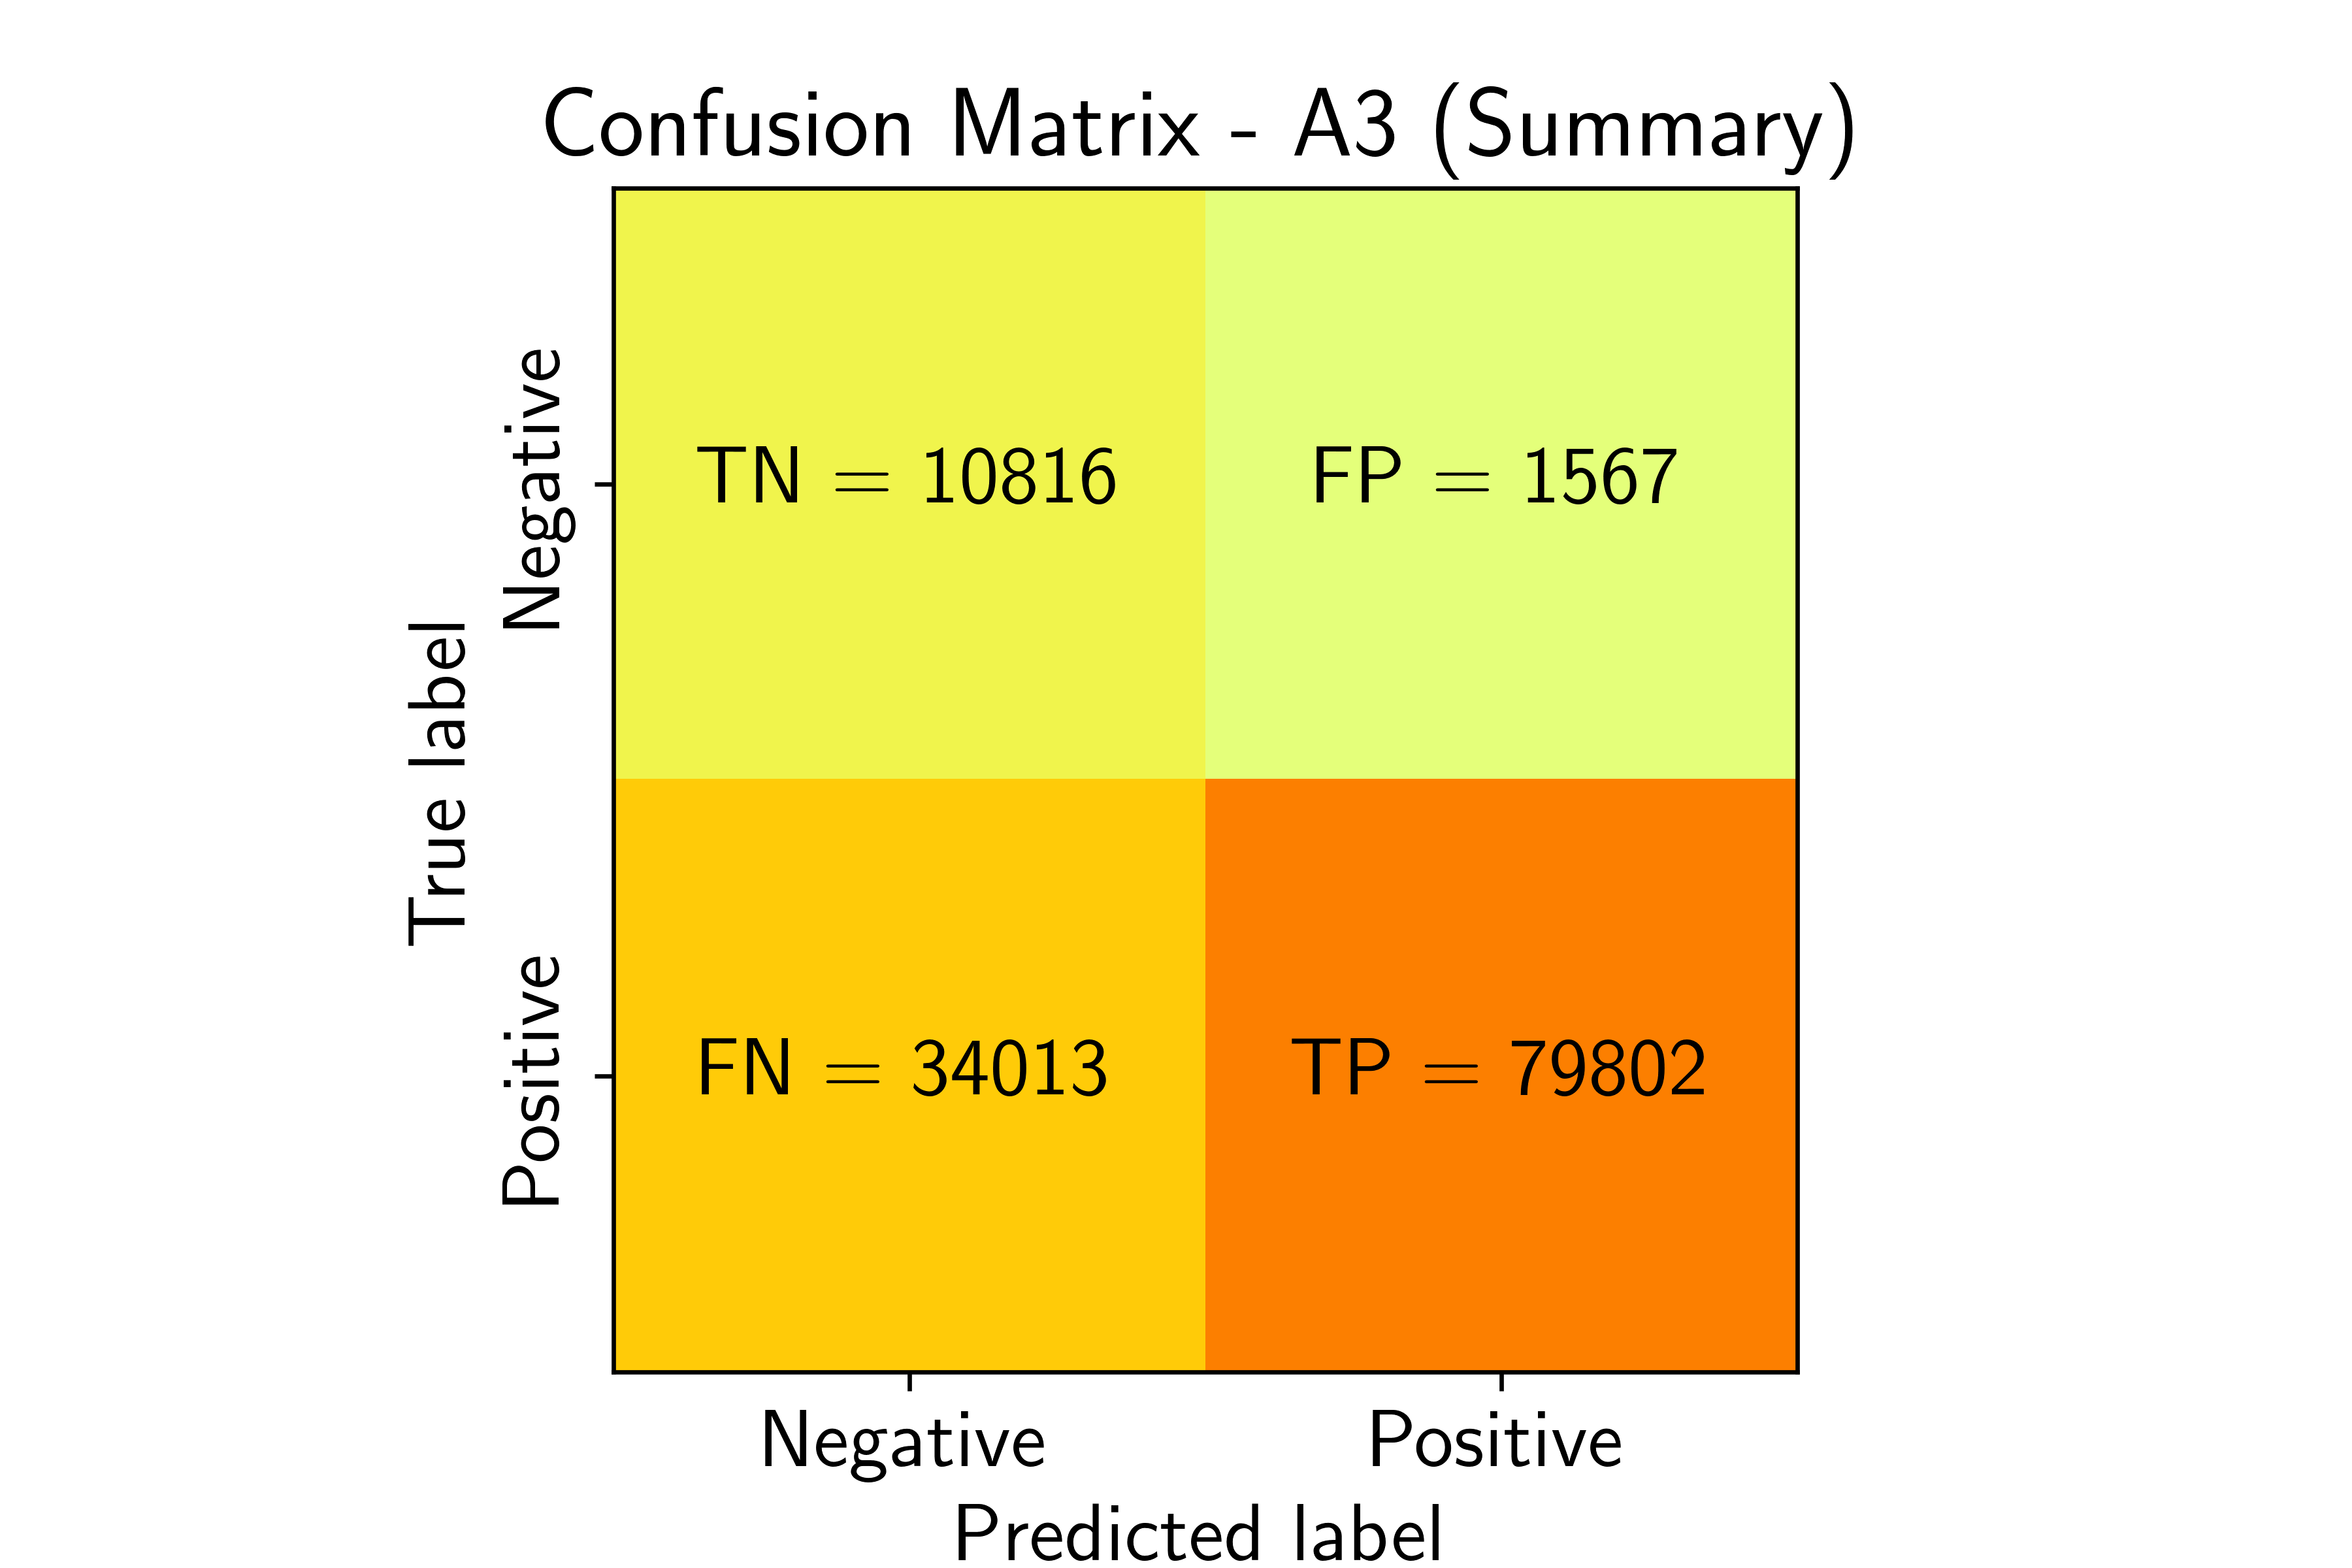
\includegraphics[width=0.48\columnwidth]{figures/Only_Metric/CMonlyA3_SUMMARY}
\end{figure}


%\section*{Additional Files}
%  \subsection*{Additional file 1 --- Sample additional file title}
%    Additional file descriptions text (including details of how to
%    view the file, if it is in a non-standard format or the file extension).  This might
%    refer to a multi-page table or a figure.
%
%  \subsection*{Additional file 2 --- Sample additional file title}
%    Additional file descriptions text.

\end{backmatter}

\end{document}
